\documentclass{article}
\usepackage[toc,page]{appendix}
\usepackage[utf8]{inputenc}
\usepackage{titlesec}
\usepackage{hyperref}
\usepackage{listings}
\usepackage{color}
\usepackage{natbib}
\usepackage{graphicx}
\usepackage{amsmath}
\usepackage[margin=1in]{geometry}
\usepackage{pgfplots}
\pgfplotsset{width=5.5in,compat=1.10}
\usepackage{setspace}
\doublespacing


\definecolor{codegreen}{rgb}{0,0.6,0}
\definecolor{codegray}{rgb}{0.5,0.5,0.5}
\definecolor{codepurple}{rgb}{0.58,0,0.82}
\definecolor{backcolour}{rgb}{1,1,1}
 
\lstdefinestyle{mystyle}{
    backgroundcolor=\color{backcolour},   
    commentstyle=\color{codegreen},
    keywordstyle=\color{magenta},
    numberstyle=\tiny\color{codegray},
    stringstyle=\color{codepurple},
    basicstyle=\footnotesize,
    breakatwhitespace=false,         
    breaklines=true,                 
    captionpos=b,                    
    keepspaces=true,                 
    numbers=left,                    
    numbersep=5pt,                  
    showspaces=false,                
    showstringspaces=false,
    showtabs=false,                  
    tabsize=2
}
 
\lstset{style=mystyle}

\newcommand\tab[1][0.5cm]{\hspace*{#1}}

\titleclass{\subsubsubsection}{straight}[\subsection]
\newcounter{subsubsubsection}[subsubsection]
\renewcommand\thesubsubsubsection{\thesubsubsection.\arabic{subsubsubsection}}
\renewcommand\theparagraph{\thesubsubsubsection.\arabic{paragraph}} % optional; useful if paragraphs are to be numbered

\titleformat{\subsubsubsection}
  {\normalfont\normalsize\bfseries}{\thesubsubsubsection}{1em}{}
\titlespacing*{\subsubsubsection}
{0pt}{3.25ex plus 1ex minus .2ex}{1.5ex plus .2ex}

\makeatletter
\renewcommand\paragraph{\@startsection{paragraph}{5}{\z@}%
  {3.25ex \@plus1ex \@minus.2ex}%
  {-1em}%
  {\normalfont\normalsize\bfseries}}
\renewcommand\subparagraph{\@startsection{subparagraph}{6}{\parindent}%
  {3.25ex \@plus1ex \@minus .2ex}%
  {-1em}%
  {\normalfont\normalsize\bfseries}}
\def\toclevel@subsubsubsection{4}
\def\toclevel@paragraph{5}
\def\toclevel@paragraph{6}
\def\l@subsubsubsection{\@dottedtocline{4}{7em}{4em}}
\def\l@paragraph{\@dottedtocline{5}{10em}{5em}}
\def\l@subparagraph{\@dottedtocline{6}{14em}{6em}}
\makeatother

\setcounter{secnumdepth}{4}
\setcounter{tocdepth}{4}

\title{DID7_detailedDesignDocument}
\author{mcdonaldgam }
\date{March 2017}

\begin{document}

\begin{titlepage}
    \begin{center}
        \vspace*{1cm}
        \textbf{Royal Military College of Canada}\\
        \vspace{0.5cm}
        Department of Electrical and Computer Engineering
        \vfill
        
\includegraphics[scale=1]{tdv_logo}
        \vfill
        \textbf{Detailed Design Document}\\
        \textbf{EEE455/457-DID-07}\\
        for\\
        \textbf{Localization Using a ROS-Based Robot}\\
        \vfill
        OCdt Michael Kogan\\
        OCdt Garrett McDonald\\
        \vfill
        \textbf{Project 16-12}
        \vfill
        Supervisor: Dr. Sidney Givigi\\
        Project Manager: Maj Peter Jardine\\
        16 March 2017
        \vspace*{1cm}
    \end{center}
\end{titlepage}

%\maketitle
\tableofcontents

\clearpage
\section{Introduction}
\tab ``Autonomous robotics has had a relationship with science fiction that is deeply rooted in our instinct to understand ourselves as primary actors in the world. Conceiving of robots that are autonomous has compelled us to build models and paradigms that are biologically inspired. The current state of the art is multifaceted. On one hand, we are equipping our machines (e.g., vehicles) with robotic gadgets (e.g., navigation tools) to make decisions on our behalf. On the other hand, we are relinquishing certain well-understood operations to robotic automation (e.g. manufacturing). We also aspire for robots that will exist in harmony with us.''
\rightline{{\rm --- Henry Mexmoor}}\citep{EPAR}\\

\subsection{Background}
\tab When deciding on a topic for our project, we knew that we wanted to work on a problem involving robotics. However, we were unsure of what exactly we wanted to do. Upon consulting Maj. Jardine, we were introduced to Simultaneous Localization and Mapping (SLAM), a field in which a robot creates a map and localizes itself on that map at the same time. We then consulted Dr. Givigi, who helped us scope our project further, directing us towards the localization problem. There is no universally accepted solution to the localization problem as the problem is far from trivial. Given a map of its surroundings, a robot must use sensor data to locate itself on the map\citep{ProbRob}.\\

The solution to the localization problem has many applications, as many robotics applications require the robot to know where it is. In order to see the importance of solving the this problem, let us look at the broader question of robot navigation. Robot navigation has a whole multitude of applications as it is applicable to autonomous robotics (robots that act by themselves). These robots can be used to explore environments that are difficult or dangerous for humans to explore. Missions to planets and outer space, or radioactive sites are just two examples of this. Another area where autonomous robotics can be useful is the entertainment sector, where robots can be used as museum guides, showing people around by navigating the exhibits. A last example is that autonomous robots could have an interesting application in the service sector, performing janitorial duties and deliveries. \\

Robot navigation has three main components, these are: localization, goal recognition, and path planning. In this project will explore the first problem, the localization aspect. You cannot have robot navigation, and by extension cannot apply autonomous robotics to real life problems, if you are unable to localize your robot within its environment. This is why solving the localization problem is so important, it is the first step in applying robots to accomplish truly useful tasks. The localization problem is one of the most fundamental problems in autonomous robotics. As a matter of fact, autonomous robotics is not truly possible without localization\citep{KalmanFilter}.

\subsection{Project Thesis or Aim Statement}
\tab The aim of this project is to implement a localization algorithm on a robot that will use its sensors and a map of its environment to determine the location of the robot. Additionally, different sampling algorithms will be compared in order to see which ones will give the best results. This is a fundamental part of robot navigation, and therefore is integral to autonomous robotics.

\subsection{Scope}
\tab The scope of this project is to design and implement a localization algorithm that will run on the Turtlebot platform. The Turtlebot is a mobile base with a Kinect sensor, and therefore has all of the tools required to solve this problem. The algorithm was implemented on top of the Robot Operating System (ROS). ROS is a software package for Linux that abstracts away a lot of the basic robotics problems, such as getting a robot to move and read sensors\citep{ROS}. The code was written and compiled in the ROS environment. The maps were be generated by hand in order to ensure accuracy. The goal was be to take these maps and to localize the robot within them, and to compare different sampling algorithms to determine which ones work best. An environment was built in the lab using a modular construction set known as Brik-a-Block. Finally, the project was considered to have worked as intended if the Turtlebot could be placed in a random location within the environment and was able to determine where it was on that map using the localization algorithm that was implemented. All of the testing was contained to the robotics lab. The localization algorithm should work just as well in any static environment in which the sensor is able to detect its surroundings. The lab environment was therefore sufficient in order to demonstrate that the algorithm worked as intended.

\subsection{Document Overview}
\tab The purpose of this document is to provide an overall discussion on the changes and deviations from the originally intended product. It will include descriptions of any changes or deviations form the original document, as well as justifications for these changes. It will also present the details of the final design project, provide all design artifacts, present the final results, provide a summary of the degree of success of this project, and provide feedback on the experience of having a final design project.

\section{Referenced Documents}
\bibliographystyle{plain}
\bibliography{references}

\section{Requirements}\label{fig:reqs}
\subsection{Functional Requirements}
\subsubsection{FR01: Movement}
The robot shall be able to move in straight line and pivot around its vertical axis using ROS’s Twist library. See PR-05 and PR-06.
\subsubsection{FR02: Sensing}
The robot shall be able to sense its surroundings through the Kinect and publish its pointcloud data so that other nodes may subscribe to it and receive that data. This data will be turned into 2D LIDAR data.
\subsubsection{FR03: Collision}
The robot shall be able to determine whether or not it has hit an obstacle.
\subsubsection{FR04: Autonomy}
The robot shall be able to perform its tasks with minimal user input. See PR-04.
\subsubsection{FR05: Localization}
The robot shall be able to localize itself in an environment given a map of that environment. See PR-01, PR-02 and PR-03.

\subsection{Interface Requirements}
\subsubsection{IR01: Wireless Control}
The robot must be able to be remotely controlled from another computer.
\subsubsection{IR02: Sensor}
The Kinect sensor must be interfaced through the USB cable.
\subsubsection{IR03: Keyboard}
The user will control the robot using the keyboard on the control  laptop.

\subsection{Performance/Timing Requirements}
\subsubsection{PR01: Fidelity of Localization in X,Y}
For the X and Y dimensions, the values must be accurate plus or minus 354mm (one superimposed Turtlebot) in any direction.
\subsubsection{PR02: Fidelity of Localization in \(\theta\)}
For the \(\theta\) value, the localization will have been successful if the robot is facing plus or minus 10 degrees of its estimated angle.
\subsubsection{PR03: Localization Time}
The device must have fully completed the localization process, resolving X, Y, and \(\theta\) within 15 seconds of being placed in order for the solution to be effective.
\subsubsection{PR04: Autonomy}
The robot will only need to be turned on initially, placed in its environment, and be given the localization command. The robot will then autonomously proceed with the localization algorithm. 
\subsubsection{PR05: Fidelity of Movement in X,Y}
The robot shall be able to move in any direction along a straight line, and be no more than 10 degrees off of its predicted line of movement.
\subsubsection{PR06: Fidelity of Movement in \(\theta\)}
The robot must be able to turn in any direction on its vertical axis and be no more than 5 degrees off the desired angle.

\subsection{Simulation Requirements}
\subsubsection{SimR01: ROS Simulation}
The code will be integrated with the Turtlebot Gazebo package.
\subsubsection{SimR02: Lab Environment}
The code will be tested using a robot in a real-world environment created in the robotics lab.

\subsection{Implementation Requirements}
\subsubsection{ImpR01: Turtlebot}
The algorithm will be implemented on the Turtlebot Create base running ROS.
\subsubsection{ImpR02: Programming Language}
The algorithm will be implemented in the Python and C++ programming languages.
\subsubsection{ImpR03: LIDAR}
The robot will use the Kinect to sense a point cloud, and then take only one slice of that pointcloud, thus creating 2D LIDAR data.

\subsection{Schedule Requirements}
\subsubsection{SchR01: Deliverables}
All documents and presentations shall be completed according to the Statement of Work.\citep{SOW}
\subsubsection{SchR02: Working Prototype}
The code will be tested using a robot in a real-world environment created in the robotics lab.

\section{Architectural Design}\label{fig:arch}
\tab As this is both a hardware and a software project, the architectural design consisted of two different designs, one for hardware and one for software. The hardware design can be seen in Figure \ref{fig:hard}.\\

\begin{figure}[h!]
\centering
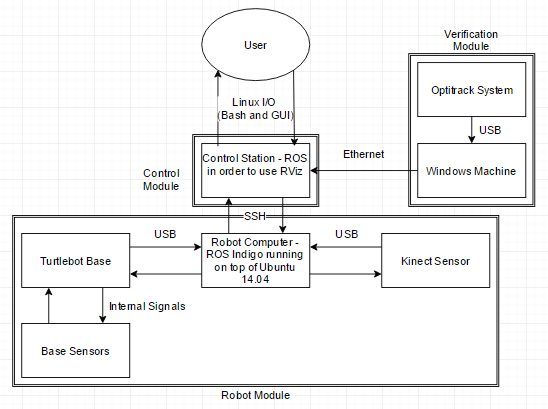
\includegraphics[scale=0.8]{hardware_arch.png}
\caption{Hardware Architecture}
\label{fig:hard}
\end{figure}

The figure above demonstrates the hardware design of the system. The user interacts with a control computer that brings together the robot and the verification modules. The robot module consists of a robot base with its internal sensors, a Kinect sensor, and a laptop to bring it all together. The verification module consists of an Optitrack system and windows computer to communicate the real position of the robot.
In addition to hardware, this project had a very large software component. The design for this can be seen in figure \ref{fig:soft}.\\

\begin{figure}[h!]
\centering
\includegraphics[scale=0.7]{software.png}
\caption{Software Architecture}
\label{fig:soft}
\end{figure}

As one can see from the figure above, the design consists of many different parts. The movement, main, and localization components were created for this project, whereas the Kinect, map server, Optitrack and visualization components already exist. One can also see that all of this runs on top of ROS, a middle-ware OS that abstracts away communication with the robot through a publisher/subscriber model. The main component receives movement commands from the movement components, reads the scan from the Kinect components, and calls functions in the localization components. It gets a map from the map server, and publishes to the visualization component (RViz) the position and the particles used. It also sends commands to the movement component for synchronization. The Kinect publishes the scan to the main component as well as to the movement component. The Optitrack publishes the real position to the visualization module for comparison. The map server also provides the map for the visualization component.

\section{Detailed Design}

\subsection{Overview}
\tab Going off of section \ref{fig:arch}, the design of this system consisted of designing the hardware and the software components for this project. The hardware consisted of three modules, each with several components. The first module, and perhaps the simplest, is the control module. This module, which can be seen near the top of figure \ref{fig:hard}, is simply how the user will interact with the system. The goal of this module is to bring the entire project to a single point from which the user can both start the localization process and visualize it as it is happening. In order to do this, it needs to talk to both the robot and the verification modules. This hardware module will be running the visualization and map server components of the software, which can be seen in figure \ref{fig:soft} above.\\

The verification module consists of an Optitrack component and a Windows machine component. The Optitrack component is the hardware that will measure the real position of the robot, for comparison with the position determined by the localization algorithm. The Windows machine component will be the component that controls the Optitrack and publish the results to the control module for visualization and comparison. The Optitrack component of the software will be running on the windows machine.\\

Lastly, the robot module consists of a laptop, a base, internal sensors, and a Kinect sensor. The laptop ties together the base and the Kinect sensor, and the base is connected to its internal components. The majority of the localization software, including the movement, main, localization, and Kinect components, will be running on the laptop component of the robot module. The Kinect module is simply the hardware that the robot uses for range sensing, and the robot base along with its sensors is what the robot uses for actuating its movement.\\

In addition to the hardware, this project has a large software component, as previously stated. The provided software components are the Optitrack, mar server, Kinect, and visualization components. The Optitrack component is the driver for the Optitrack hardware, it allows us to accurately track the position of the robot and publish it to the visualization component. The map server component will simply distribute the information about the current map, as it is used by both the visualization component and the main component. The Kinect component is the driver for the Kinect hardware. It allows us to read sensor data from the Kinect. Lastly, the visualization component is a program that allows us to observe the functioning algorithm.\\

In addition to using already written components, three major components were written. The main component is the software component that brings everything together and runs the algorithm. It interacts with almost every other software component. The localization component contains all of the functions necessary for running the algorithm. The main component is only one function, and for all the functionality it refers to functions in the localization component. Lastly, the movement component makes movement decisions, and publishes them to the main component.\\

It is important to note that all of this software runs on top of ROS. ROS is a middle-ware operating system that abstracts away basic robotics problems, such as communication with the robot. This allows us to focus on high-level code while not having to worry about writing controls for simple things such as movement and sensor reading. ROS uses a publisher-subscriber system, meaning messages are published to topics and read from topics. However, there is also a way to wait for a single message without specifying a topic using ROS system calls. ROS and the publisher-subscriber system are described in further detail in the ROS section \ref{ROSMod} of this document.\\

\subsection{Limitations}
\subsubsection{Movement Update}
\tab The movement update step of the MCL algorithm requires us to provide it with a movement update at each iteration. The movement update consists of a linear velocity, an angular velocity, and a time duration (how long the velocities are applied for). The problem that was run into is that it is not possible to determine with complete certainty how long the movements are applied for, since the drivers are abstracted away. The solution is to approximate this by applying the movement update several times and roughly timing how long each update takes, and then averaging those numbers to come up with a close, but not completely accurate estimate for the duration of time that each movement update is applied for. Additionally, this estimate is only accurate for the Turtlebot, and will not be accurate for other platforms.
\subsubsection{Environment Type}
\tab This project focuses on localization in a static environment. This means that the initial map of the environment is a completely accurate representation of the environment at any point in time. There cannot be people walking around or any other unexpected sightings, or the localization algorithm may fail. This was done in order to scope the project in the beginning, but working in dynamic environments is definitely an attainable amendment for future work.
\subsubsection{Map Accuracy}
\tab In order for this localization algorithm to work, the map has to be completely accurate; any small errors will throw the algorithm off. This means that maps have to be hand-made, and cannot be made using mapping software like originally intended.  This means that usability in the real world may be limited for now as perfect maps are very time-consuming and difficult to make, most maps are constructed using mapping software.
\subsection{Module Descriptions - Software}
\subsubsection{ROS} \label{ROSMod}
\tab ROS is the middle-ware operating system on which this whole project is based. The intent of ROS is to remove the need for programmers to worry about the basic details of robotics, such as movement and sensor readings, and allow programmers to focus on developing writing high level code instead. Just like any other operating system, it makes the underlying hardware easier to program and simplifies the life of the programmer. It also adds portability. If code works on one robot, and it is written in ROS, it should theoretically work on any other ROS-based robot.\\

ROS is based off of the publisher-subscriber model. This model is relatively simple. Each running program is called a node. This can be seen as a process. Every node, in order to be useful, needs to communicate with other nodes. Communication is done by publishing messages to topics, or by subscribing to topics and receiving information on callbacks. When a node publishes a message to a topic, it is sent to the incoming message queue of every node that has subscribed to the topic, and this message stays in that queue until it is read by the receiving node. A good way to visualize this is through mailboxes. Each node has one mailbox for each topic it is subscribed to, and mail is picked up from the mail box in the order it is received, a first-in-first-out system. Messages are only read from the mailbox when they are picked up in a callback function, a function written specifically to pick up these messages from the corresponding message queues. Each message queue therefore has a corresponding callback function. Figure \ref{fig:pubsub} provides a visualization of this.\\

\begin{figure}[h!]
\centering
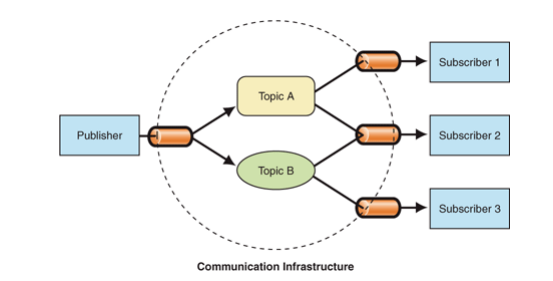
\includegraphics[scale=0.8]{pub_sub_model.png}
\caption{Publisher Subscriber Model}
\label{fig:pubsub}
\end{figure}

Using ROS instead of coding from scratch allowed the reusing of a lot of code previously written, not in order to accomplish the task, but in order to build the correct infrastructure necessary for this project. All of the modules except for main, localization, and movement have nothing to do with localization itself, yet are vital for the project because of the services they provide. This is why ROS was chosen as the middle-ware for this project.


\subsubsection{Main}
\subsubsubsection{Main Component Design Specification and Constraints}
\tab The requirement for this component is to tie together the entire project while running the localization algorithm. This means it has to accept the map, movement and sensor updates, and run the algorithm using those updates, as well as format the results of each step of the algorithm so that it may be visualized by the visualization component. This module has the following inputs/outputs:

\begin{figure}[h!]
\centering
 \begin{tabular}{||c c c c||} 
 \hline
 Input & Related Component & Output & Related Component \\ [0.5ex] 
 \hline\hline
 /map & Map Server & /particles & Visualization \\ 
 \hline
 /scan & Kinect & /position & Visualization \\
 \hline
 /move & Movement & /sync & Movement  \\
 \hline
 Function Call Results & Localization & & \\ 
 \hline
\end{tabular}
\caption{Main I/O Specifications}
\label{fig:MainIO}
\end{figure}

\subsubsubsection{Main Component Design}
\tab The main component followed the universally-accepted standard for main components, being a single function called int main(int argc, char **argv). This single function is the piece that ties the entire project together. It collects data from other components, and calls upon the functionality of others to achieve its objective, all the while remaining a very high-level piece of code in the sense that all the details are handled by the other components, the main component simply deals with the high-level algorithm.\\

As mentioned before, the main component will be running the localization algorithm. The algorithm that was chosen for localization is the particle filter based Monte Carlo localization algorithm. This algorithm is a probabilistic algorithm based off of recursive Bayesian estimation\citep{ProbRob}. What this means is that the location of the robot is estimated over time using incoming measurements and a movement model for the robot. The algorithm in its generic form can be seen in figure \ref{fig:mcl}.\\

\begin{figure}[h!]
\centering
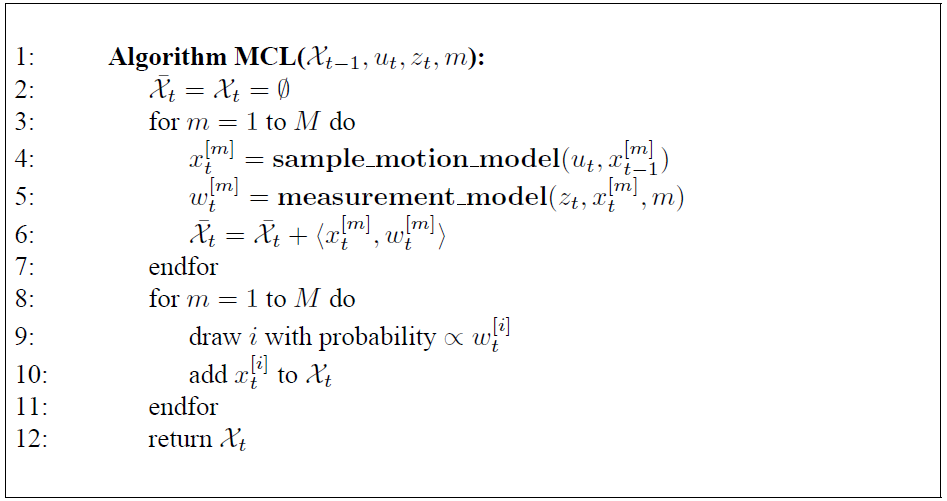
\includegraphics[scale=0.45]{mcl_algorithm.png}
\caption{MCL Algorithm}
\label{fig:mcl}
\end{figure}

The first step is to distribute the particles. A particle is a guess, so given a map, N particles would be distributed, each with a random x-coordinate, y-coordinate, and orientation. The next step is to make a movement decision. This is done by the movement component. Once the movement command has been made, the robot will move. The movement update is also applied to each one of the particles, adding in uncertainty to compensate for the fact that movement is almost always imperfect\citep{ProbRob}. The movement model is described in detail in the next component, Localization. Next the sensors are read, and each particle is assigned a weight based on what it is seeing and what it should be seeing.  This again is described in detail in the next section, Localization. This means that likely particles, or good guesses, are assigned a high weight, whereas bad guesses are assigned a low weight, since the sensor reading does not match that which would be seen at their position. Once each particle has a weight, a cumulative distribution function (CDF) is constructed. This is done by first finding the normalizing factor, which is the sum of all the particle weights, and then constructing an array where each element is equal to the sum of the weights up until that element divided by the normalization factor, or
\[CDF_n = \sum_{i=1}^{n} \frac{ParticleWeight}{\eta}, \textrm{where }{\eta}\textrm{ is the normalization factor} \]
\tab The CDF is used to re-sample the particles. The particles are re-sampled using a re-sampling algorithm; which requires the list of particles and the CDF. Different re-sampling techniques are covered in the next component, Localization. Once re-sampled, the particles will converge towards those with more likely values. This is because the CDF will see spikes in areas where the weight was high, and the re-sampling uses that to redistribute the particles accordingly.\\

One important problem that exists in localization is the kidnapped robot problem\citep{ProbRob}. This problem occurs when a robot has already localized, but is then picked up and moved somewhere else. This means that all of the particles, or guesses, are located in the previously believed guess, but the robot is in a completely different spot. Since there are no particles where the robot is now, because they are all clustered around where it was before, the robot is unable to re-localize itself. In order to solve this problem, the main component also checks the normalization factor that was calculated before the CDF. This normalization factor is the sum of all the weights. If there are no high weights, meaning no good guesses, it would mean that no particles are in the right area. This concept was used to solve the kidnapped robot problem. If the normalization factor is below a certain threshold, then the particles are redistributed. This solves the kidnapped robot problem.\\

The last goal of the main component is publish the results of each step of the algorithm to the visualization software. This done by calling functions in the Localization component that will use the list of particles in order to generate messages allowing us to visualize the particles and the current location.
\subsubsection{Localization}
\subsubsubsection{Localization Component Design Specifications and Constraints}
\tab The requirement for this component is to provide all of the necessary functionality to the main component so that the main component may run the algorithm at a high level. This component had to provide functionality to run the movement model, the measurement model, the re-sampling code, and all the supporting framework. This section will detail the movement model, the measurement model, and the re-sampling code. The supporting functions are not explained in detail, however, the code and comments that describe them can be found in Annex \ref{fig:mclcode}. This component’s only inputs are function calls with parameters, and the only outputs are the returns from these function calls.
\subsubsubsection{Localization Component Design}
\tab This component of the software is simply a bank of functions that the main component could rely on in order to complete its localization. As such, it was designed as a header file that contained all of the constants, structure definitions, and function prototypes, and a code file that implemented these functions. The component itself contains over twenty functions, most of which are there to help the three main functionalities that this component provides. These are the movement model, the measurement model, and the re-sampling function. These will be described in more detail in this section.\\

The first part of the MCL algorithm involves applying a movement update to each particle. Although the simple solution would be to take the particle and project its position using the movement update, uncertainty needs to be added to the movement in order to ensure that environmental factors are covered. Anything from a wheel slipping to hitting an obstacle could cause the robot to not move exactly as predicted, and as such, uncertainty needs to be added each time a particle’s future position is projected using the control input. This process is called the movement model, as it models the motion of the robot given a control input, while adding uncertainty to model real-world events. The algorithm for this can be seen if figure \ref{fig:motion}.\\

\begin{figure}[h!]
\centering
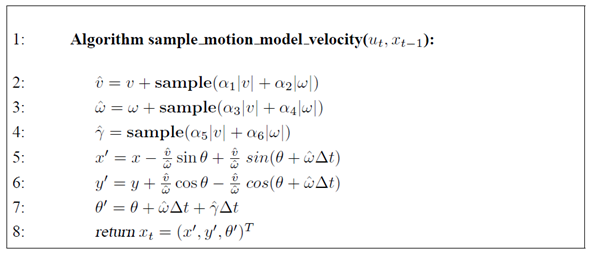
\includegraphics[scale=0.75]{motion_algorithm.PNG}
\caption{Motion Model}
\label{fig:motion}
\end{figure}

As one can see, the motion model calculates each particle's linear and angular velocity by adding uncertainty to the control linear and angular velocities\citep{ProbRob}. It also calculates a small angular uncertainty. Lastly, it applies these “real-world’ velocities to the current position to obtain the new position. Please note that the coefficient a1 through a6 are simply chosen so as to best represent the real-life scenario. Since the motors are rather accurate, these values were chosen to be relatively small. However, if the motors were not as accurate, these values would be chosen to be much higher. The sample function simply samples a normal distribution according to the following equation.
\[sample(x) = \frac{x}{6}\sum_{i=1}^{12} rand(-1,1),\textrm{where rand(a,b) generates a random uniform number between a and b} \]
\tab For the movement model, the map of the environment was also taken into consideration, not letting any particles move into walls, and if retrying five times failed then the particle would be given a random location on the map, because it was clearly in an incorrect spot if it is unable to perform the motion update.\\

The other model that was implemented for this project was the measurement model. This involves assigning each particle a weight based off what is currently being seen by the sensor. This means taking what is being sensed by the Kinect and comparing it to what each particle should be seeing. Then based off the comparison of those two, coming up with a model that would nicely assign weights to each particle. Since the robot performs a beam range finder scan, the measurement model was based off the beam model. The algorithm for this can be seen in figure \ref{fig:range}.\\

\begin{figure}[h!]
\centering
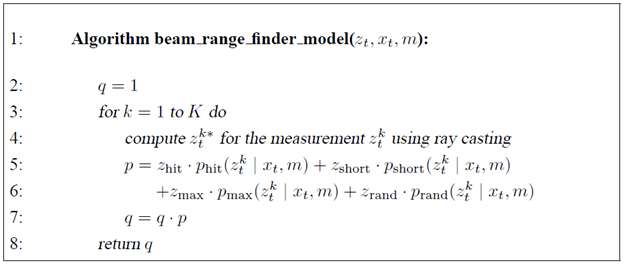
\includegraphics[scale=0.70]{range_algorithm.PNG}
\caption{Measurement Model}
\label{fig:range}
\end{figure}

As one can see, the measurement model does assign a nice weight to each particle. It does so by first initializing the weight to one. Then, for each measurement from the beam finder, it compares the measurement that is sensed to that which is projected for the given particle. The projected measurement is what the particle should be seeing given that it is in the position that it is. Then, it calculates a value for that particular measurement in the beam model. This value is calculated as a weighted average of four different components. The first, and the most important, is how likely the actual measurement was. This is calculated using a normal distribution, and in this model, it is given a weight of 95 percent, so the actual measurement accounts for 95 percent of the weight for that particular measurement. Next, there is a probability of a short measurement, meaning there is an object in the environment that is not expected. This is not applicable to this project since only static environments are considered, so the value of that is set to zero. The next one is the probability that the maximum possible range is sensed. This is given a small probability weight of five percent, as it is rather unlikely in the tested environments that there will be values sensed that hit or exceed the maximum sensor range. Lastly, there is a random measurement probability. This measurement was given a weight of zero because random measurements are not applicable to the implemented model. Essentially what the implemented variation does is calculate the weight of the projected measurement relative to the actual measurement, and then multiplies that by 0.95 and adds 0.05 if the maximum possible range is sensed. This measurement model proved to work quite well during testing.\\

The last major functionality that this component provides is the re-sampling algorithm. The purpose of this algorithm is to take the set of particles and the cumulative distribution function, and to redistribute the particles so that the particles with low weights shift towards those with high weights. The first re-sampling algorithm that this component provides is the basic re-sampling algorithm, called uniform re-sampling\citep{ProbRob}. This algorithm goes through each particle, and for each particle calculates a random uniformly distributed double and finds the first element in the cumulative distribution function array that is equal to or greater than the randomly selected double. It then sets the position of the current particle equal to the position of that whose index matches the one found in the cumulative distribution array. This works because this algorithm redistributes particles to those positions where there was a spike in the cumulative distribution function, and the spikes occur where there were high weights, so the particles are shifted towards those with high weights. To better understand this, one may look at the following example with ten particles, each with a given weight:\\

\begin{figure}[h!]
\centering
 \begin{tabular}{|| c | c || c | c ||} 
 \hline
 Particle 1 & Weight 0.1 & Particle 2 & Weight 0.05 \\
 \hline
 Particle 3 & Weight 0.01 & Particle 4 & Weight 0.02 \\ 
 \hline
 Particle 5 & Weight 0.03 & Particle 6 & Weight 0.04 \\
 \hline
 Particle 7 & Weight 0.05 & Particle 8 & Weight 0.2 \\
 \hline
 Particle 9 & Weight 0.4 & Particle 10 & Weight 0.1\\
 \hline
\end{tabular}
\caption{re-sampling Example}
\label{fig:resample_ex}
\end{figure}

\begin{figure}[h!]
\centering
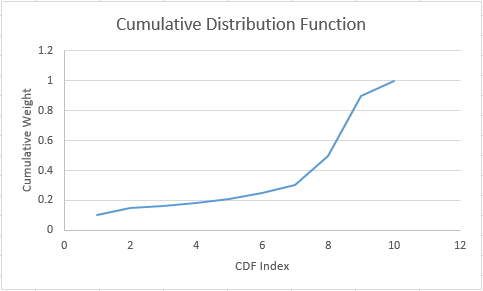
\includegraphics[scale=1.0]{cum_sum.PNG}
\caption{Cumulative Distribution Function Example}
\label{fig:cum_sum}
\end{figure}

The cumulative distribution function for this can be seen in figure \ref{fig:cum_sum}. At this point, the particles are iterated over, and for each particle, a random number is generated. It is evident that all random numbers that hit between 0.5 and 0.9 will be distributed to the position of particle 9, which had a weight of 0.4. This means that the number of particles at each location after the re-sampling will be proportional to its weight, so the particles will naturally migrate towards those particles with higher weights.\\

The second re-sampling algorithm that was implemented is known as KLD sampling. The advantage of this algorithm is that it changes the number of particles that are used as the localization gets better, thereby increasing the performance of the algorithm in the long term by reducing the number of particles over time. This increases the speed at which the algorithm is running by reducing the computational complexity\citep{ProbRob}. Although this algorithm certainly increases performance in the long run, it remains to be seen if it will prove to be the better of the two algorithms. This algorithm works much like the previous one in terms of using the CDF. It will still pick particles and place them in locations that are deemed more likely by looking at the CDF. However, the difference is that it will also calculate how many particles are needed as it is re-sampling\citep{KLD}. The algorithm for this can be seen in figure \ref{fig:KLD_re-sampling}.\\

\begin{figure}[h!]
\centering
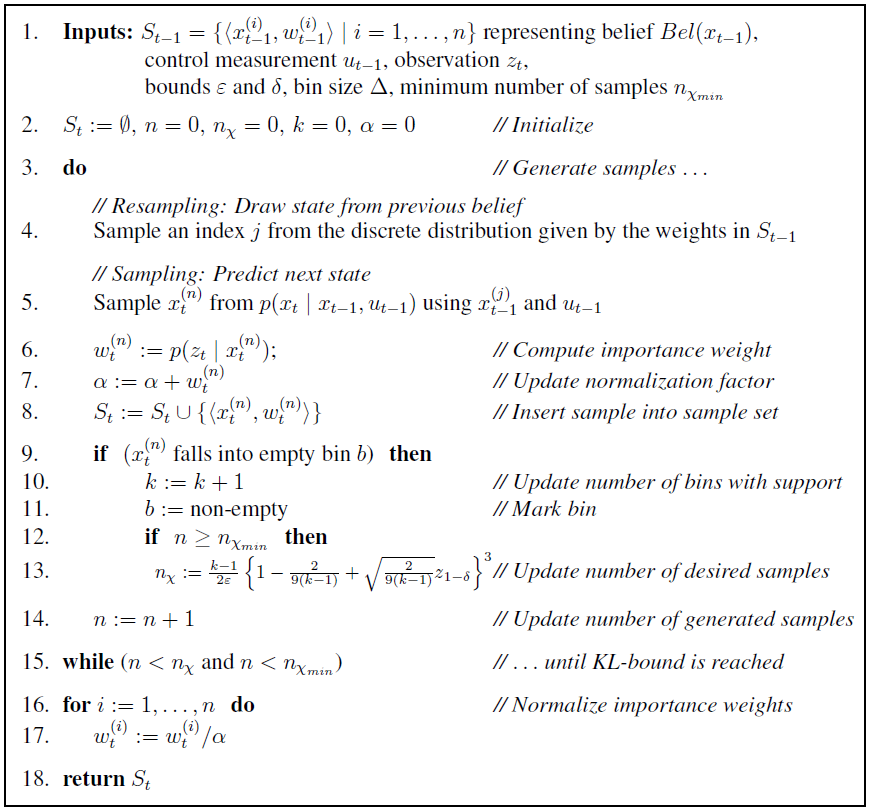
\includegraphics[scale=0.4]{KLD_Algo.PNG}
\caption{KLD re-sampling Algorithm}
\label{fig:KLD_re-sampling}
\end{figure}

This algorithm dynamically calculates the number of particles required to achieve a good approximation. A good approximation is defined as a distribution, $q(x)$, where the Kullback-Leiber distance (KL-distance) from the the distribution that is approximated, $p(x)$, is no more than $\epsilon$, with a certainty of $1 - \delta$\citep{KLD}. The KL-distance between two distribution is calculated as follows: $K(p, q) = \sum_{x}p(x)log\frac{p(x)}{q(x)}$\citep{KLD}. This fact was used in order to calculate the KL bound, or how many particles are needed to approximate the true distribution. Particles were then added until the minimum amount or the KL bound was reached, whichever comes last. This means that at least the minimum number of particles was generated, and potentially more if more is needed in order to approximate the distribution well. The KL-bound was also given a ceiling value, so as to not generate obscene number of particles, thereby removing the benefit of using this type of re-sampling. In practice, this re-sampling method is quite simple to implement given the previous set of particles and the CDF.\\ 

At first, the map was split into bins, or large areas. These areas were chosen to be 50cm by 50cm by 10 degrees sections. Then, a desired $\epsilon$ and $1-\delta$ were chosen. In this case, the values were $\epsilon = 0.05$ and $1-\delta = 0.99$. Now that the values had been chosen, the do-while loop would be executed, until the minimum number of particles was hit, and if the KL bound was more than the minimum number of particles, the loop was executed until the KL-bound was hit. However, the loop was only executed up to the number of times that is dictated by the ceiling value placed on the KL-bound. At each iteration, a particle would be drawn and added to a new set. Then, it was determined whether or not the particle had fallen into an empty bin. If so, the number of active bins would be incremented, the bin would be marked as non-empty, and if the number of particles was greater than or equal to the minimum number of particles, the KL-bound was calculated. What this means in practice is that there is no point in calculating the KL bound until at least the minimum number of particles has been reached, because the KL-bound is irrelevant until at least the minimum number of particles was reached. The KL bound was calculated using the following formula:\\ $$KLB = \frac{k-1}{2\epsilon}\Bigg\{1 - \frac{2}{9(k-1)} + \sqrt{\frac{2}{9(k-1)}}z_{1-\delta}\Bigg\}^3\textrm{, where k is the number of active bins}$$

Please note that in the equation above, there is a term $z_{1-\delta}$, which is simply the z-table value corresponding to the $1-\delta$, so in this case, $z_{1-\delta} = z_{0.99} = 0.83891$. The formula above is actually an approximation of the quantiles of the chi-squared distribution, given by the Wilson-Hilferty transformation\citep{KLD}. Upon running the KLD algorithm multiple times, it was discovered that the relationship between the number of bins and the number of generated particles is almost linear, despite the fact that the formula to calculate the number of particles based off of the number of bins is complex and computationally expensive, involving square roots and exponentiation. As such, a linear approximation was used for calculating the number of particles. To do this, the number of particles for 2 bins, for 10 bins, for 20 bins, and so on until 1000 bins was calculated, all using the Wilson-Hilferty transformation above. This generated a large data set for the number of bins and corresponding KL-bound values. 1000 bins was chosen as the maximum because in practice this number was never exceeded. A plot was made in excel, and using Excel's curve-fitting feature, the data was fit to a line. The corresponding equation was: $KLB = 10.303k + 86.245\textrm{, where k is the number of active bins}$. The $R^2$ value was one, which means that the approximation is a very good one. The curve can be seen in figure \ref{fig:KLD_approximation}.\\

\begin{figure}[h!]
\centering
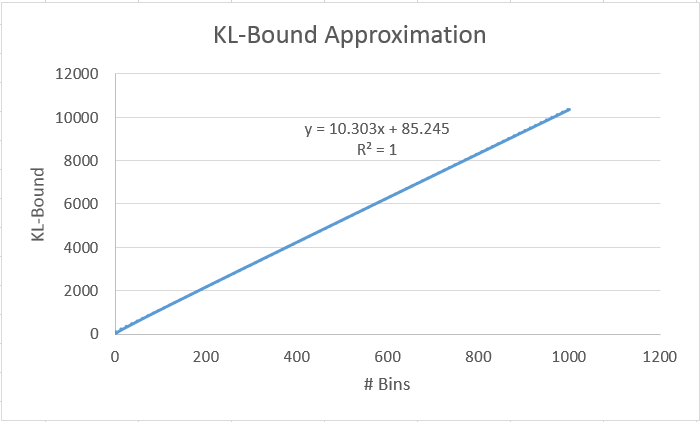
\includegraphics[scale=0.75]{KLD_Apro.PNG}
\caption{KLD Approximation Curve}
\label{fig:KLD_approximation}
\end{figure}

The KLD Sampling method evolved the particles over time, starting with a high number, usually hitting the ceiling value of 1000, staying there for a few iterations, and then rapidly decreasing as time went by. Although this general pattern was followed, every situation is different. Not only is this algorithm being run against different maps in different environments, the particles are distributed randomly. This means that when running the same algorithm with the exact same initial conditions, the evolution of the particles could be different due to the random nature of the initial dispersion of particles. Figure \ref{fig:KLD-evolution} shows a graph of the evolution of the number of particles in a typical localization scenario, as well as the number of bins and the true KL-bound.\\

As one can see from figure \ref{fig:KLD-evolution}, the number of particles initially should be close to 3750, but in order to improve performance the KL-bound was capped of at 1000. As the robot proceeds to localize itself, the number of bins decreases, and in a few steps there is a noticeable difference in the number of particles generated. The number of particles generated will match the value of the KL-bound up until the point where the KL-bound starts to dip below 500, which is set as the minimum number of particles in order to ensure accuracy. The curve also shows the number of bins decreasing quickly over time, explaining why the particles drop in number so quickly. The true particle count will always be bound by the particle limit and the minimum allowed number of particles.

\begin{figure}[h!]
\centering
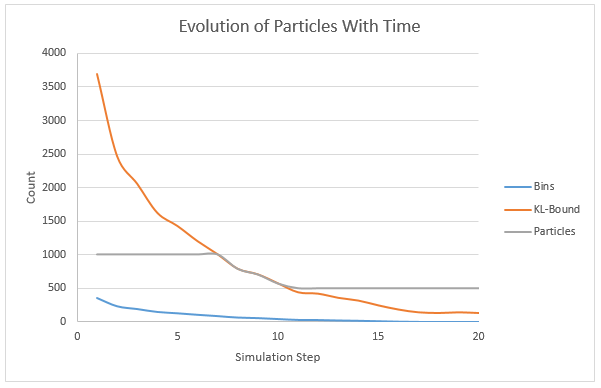
\includegraphics[scale=0.9]{KLD_Evo.PNG}
\caption{KLD Particle Evolution}
\label{fig:KLD-evolution}
\end{figure}

\subsubsection{Movement}
\tab Having multiple methods for moving a robot is important for localization. Devices that use localization typically do so alongside another primary task. This primary task may require the robot to move in a specific way, so it is important that the localization module accommodates a variety of possibilities for moving the robot. While not directly a part of the Monte Carlo algorithm, the way in which the Turtlebot moves changes how effectively and efficiently it is able to localize. The localization algorithm was ran alongside three different methods for motion. The movement function would publish it's messages in sync with the main component running the algorithm. In order to do this, a synchronization message was sent every time the main component was ready to receive a movement update. This would tell the movement component to publish the current movement message and prepare the next one. Synchronization messages are simply empty strings sent by the main component. This can be visualized in figure \ref{fig:sync}.\\

\begin{figure}[h!]
\centering
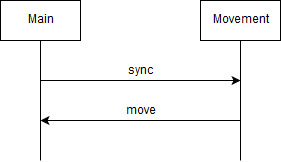
\includegraphics[scale=0.75]{Sync.jpg}
\caption{Main-Movement Synchronization}
\label{fig:sync}
\end{figure}

\subsubsubsection{Remote Control}
\tab The first way in which the robot may move, is using remote control from a user. This method of movement requires the user to have a computer with a keyboard and a wireless connection to the robot console. The robot prompts the user for an input of w, s, a, or d in the console and then moves forward, moves back, turns left, or turns right respectively. This method for controlling the robot is not optimal. Waiting for user input can substantially slow the localization process. As well, in order to implement this, the console is swapped out, so as to disable console echo and make it so that a key is processed as soon as it is typed, without having to wait for the user to press the enter key. The console is restored once the user exited the remote control using the x key.\\

These factors make remote control far from ideal for localization, however it is still an important movement function to have. Many common electronic devices work off of remote control and user input. It is possible that one of these appliances would also run a localization algorithm, making this method of movement practical. Furthermore, this motion is the easiest to observe and analyze in the lab as the user can easily pause and continue movement as they wish. This allows the user to better analyze the changes in the particles in the Turtlebot's new position. Finally, there are certain scenarios where this method of movement is actually preferred. If in a particular room the robot takes long to localize, remote control allows the user to drive the robot to a location within the room where the robot may localize more easily, such as a unique location on the map.\\

Unlike the Automated Movement and Movement to Objective functions, the Turtlebot does not stop itself from running into obstacles under when moving via remote control. This is meant to be the option for motion in which the user maintains total control of the robot. This restriction is often absent in remote controlled appliances for this reason.
\subsubsubsection{Automated Movement}\label{fig:autom}
\tab In order to avoid waiting for user input, and unnecessary interfacing with the console, a possibility for moving the Turtlebot is to have it decide on its own where to move during the Monte Carlo loop. The automated movement function used by the Turtlebot has it check for obstacles, advance forward if it safe to, and turn left if moving forward is not an option. This does not move the robot in any sort optimized fashion, but instead has the robot move throughout the environment while avoiding obstacles and simultaneously localizing. This method is effective, but could likely be made much more effective if an algorithm was written that uses the map to determine the optimal movements for the robot to localize more quickly. The possibility for future work here is discussed more in section \ref{fig:fwpathing}.\\

For autonomous movement it is critical that the robot is able to navigate around obstacles. If it was to attempt to drive forward while against a wall, internally the robot would believe it had moved forward and the MCL Motion Model would update the positions of the particles accordingly. This would destroy any progress the robot had made in determining its position. Figure \ref{fig:blind} shows that, because the Turtlebot only scans a 60 degree arc and places its camera near the rear of the structure, there is a blind spot on the left and right sides of the robot preventing it from seeing certain obstacles up to 19cm in front of where it would attempt to move. A flaw of the autonomous movement module is that if the robot does not see an obstacle in this small blind spot, such as a wall corner, the robot will hit the wall and update the particles as if this had not occurred. This will upset the localization process and, in some cases, the Turtlebot will treat this as a kidnapped robot problem and restart localizing. However, this error is unlikely since the blind spot is small relative to the environments in which the the Turtlebot navigates, and was almost negligible when automated movement was tested.\\ 

\begin{figure}[h!]
\centering
\includegraphics[scale=0.8]{TurtlebotBlindSpot.png}
\caption{Turtlebot Scan Arc and Blind Spot}
\label{fig:blind}
\end{figure}

This option for motion is critical because it allows the robot to prove its ability to localize autonomously. That is to say, even though the robot is not moving along an optimized path, it will always localize itself under reasonable conditions. The ability to localize autonomously is inherently necessary to the requirements of this system, however it is also important to the project because it allows the kidnapped robot problem to be tested. The kidnapped robot problem involves moving a robot that has found its location to a new location and seeing if it is able to again find itself. The requirements for solving this problem require that the robot act autonomously. While solving this problem is not needed for the project to be functional, the Turtlebot's ability to withstand the kidnapped robot problem demonstrates the robustness of the system.\\

\subsubsubsection{Movement to Objective}
\tab This method of movement can be thought of as a hybrid between the other two. In this function, the Turtlebot moves towards a target in the environment. Specifically, the code has the robot gravitate to the colour red while avoiding any obstacles in the way. In this way a user can set the path for the robot using a red laser pointer to mark a location in the environment.\\

To move the robot, this requires two major functions. The first is to target the specified colour (currently red, however this is easily changed) and the other controls the motors based on the location of the target. Targeting the laser pointer is done by sweeping the Turtlebot's RGB camera and comparing values returned to a spectrum of colour specified using Hue, Saturation, and Lightness (HSL) values. This function returns a Boolean as to whether or not the colour was detected, as well as how far left or right the colour was in the robot's field of vision. Similar to obstacles, the robot's ability to detect the colour here is limited by the 60 degree arc of its camera.\\

The second major function controls the motors using the outputs from the targeting function. If the colour was not seen, the function proceeds to the end and repeats, and does so until the colour is detected. This keeps the function in an infinite loop where a movement update does not occur unless the colour is seen. In such a case where motion does not occur, no movement velocity is published and no sync message is received as shown in Figure \ref{fig:sync}. Instead, the localization algorithm continues to wait for a velocity to be published and only sends the sync message when a velocity is received. If the colour is detected, the robot proceeds to move and publish velocity in a similar way to the autonomous movement module. The robot determines the necessary angular velocity to best align with the target colour, and only publishes a linear velocity if no obstacles are detected by the robot sensors. This method of obstacle avoidance is subject to the same blind spots described in section \ref{fig:autom}.\\

This motion module is ineffective if the colour being used (red, however this is easily changed) exists naturally in the environment as the robot will want to move towards any occurrence of the colour. However, if this problem is avoided then controlling the robot with a laser pointer becomes a viable alternative to remote control via keyboard.\\

\subsubsection{Map Server}
\tab This component is used for serving the /map topic to the rest of the components. It reads in a map stored as a .yaml and a .pmg file, converts it to a message of type occupancy grid, and constantly publishes it to the /map topic, allowing all other components to always have access to the map if they need to. Although not difficult to write, this component was outside the scope of this project. As such, the built-in map server from ROS was used, so no design took place except for how to integrate it into the project. Integration was simply facilitated through ROS’s publisher-subscriber system, so this component was easily integrated into the project.

\subsubsection{Kinect}
\tab The driver for the Kinect is used to publish the sensor data so that other components have access to the sensor info. It takes data from the Kinect and publishes it to the /scan message so that it is in ROS-readable form. Again, writing the drivers for the Kinect is not the goal of this project, so a node from the ROS library was used to do this. Again, integration was facilitated through ROS’s publisher-subscriber system.

\subsubsection{Visualization}
\tab The visualization component is used to visualize the results in a nice graphical user interface. This functionality is again outside of the scope of the project, and it makes no sense to rewrite visualization software. As such, the currently accepted as the currently accepted standard of RViz was used. This software subscribes to topics and visualizes them nicely. It draws the map that it gets from the map server, and all of the particles and positions that it gets from the main component. Integrating it into the project was again incredibly simple due to ROS’s publisher-subscriber model.

\subsubsection{Optitrack}
\tab The last software component is the Optitrack driver. This is used to read Optitrack data and publish it to RViz. This was used to allow visual comparison between the actual position as measured by Optitrack with that determined by the localization algorithm. This component was again provided through ROS, and integrating it was easy due to ROS’s publisher-subscriber model.

\subsection{Module Descriptions - Hardware}
\subsubsection{Control Module}
\subsubsubsection{Control Module Design Specifications and Constraints}
\tab The control module is the module responsible for tying everything together for the user. Its purpose is to provide the user with an interface to the robot from which the user can run the algorithm and watch the results unfold on RViz. As such, the control module has to be a computer running Linux with ROS installed on it in order to be able to tie everything together. The diagram for the module can be seen in figure \ref{fig:cont_mod}.\\

\begin{figure}[h!]
\centering
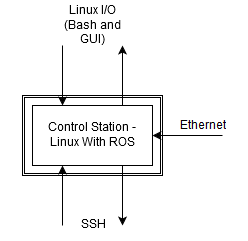
\includegraphics[scale=0.70]{control_module.PNG}
\caption{Control Module}
\label{fig:cont_mod}
\end{figure}

The control module communicated with the user via Linux, communicates with the verification module via Ethernet, and communicated with the robot module via SSH.
\subsubsubsection{Control Module Design}
\tab The design for the control module was not too involved. In order to meet the requirements of being able to visualize ROS data, this had to be a Linux-based module with ROS running so that the information could be tied together. It communicates to the robot via SSH because that provides wireless connectivity and control over the robot module, and the reason it communicates with the verification module via Ethernet is because that is the framework that is laid out in the lab, and is the only interface to the Windows machine that controls the verification module.
\subsubsection{Robot Module}
\subsubsubsection{Robot Module Design Specifications and Constraints}
\tab The robot module is responsible for running the localization algorithm and passing the results back to the control module. This module has to run ROS because that is the middle-ware on which the code is written, and it has to have wireless connectivity to be able to communicate with the control module. This means that it has to have wireless connectivity. As such, the Turtlebot was chosen for the robot module. The Turtlebot consists of four main components, which include the base itself, internal sensors and actuators, the Kinect sensor, and a robot laptop that ties this module together. The diagram for this module can be found in figure \ref{fig:rob_mod}.\\

\begin{figure}[h!]
\centering
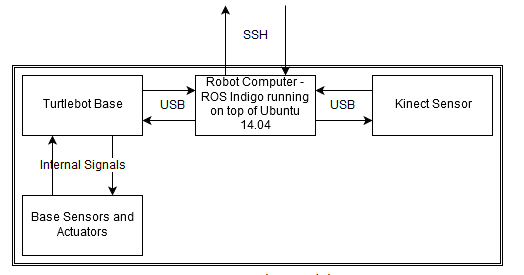
\includegraphics[scale=0.70]{robot_module.PNG}
\caption{Robot Module}
\label{fig:rob_mod}
\end{figure}

The robot module communicates to the control module via SSH. Internally, the computer communicates with the base and with the Kinect through USB, and the base communicates with its internal sensors and actuators through internal signals that are abstracted away from us.
\subsubsubsection{Robot Module Design}
\tab The design of the robot module was rather simple. Since a ROS-based robot had to be used, few choices were available which included the Turtlebot and the husky. However, it was preferred to have a platform with a laptop that is easy to work on. As such, the Turtlebot platform was chosen. This platform provides the flexibility of using a Kinect, which has many different signal types, as well as programming on a widely used platform for which many tutorials and help is available. Additionally, the husky is a much more expensive tool and is perhaps too much for the scope of this project. Once the Turtlebot platform was chosen, there was no more design to be done, as the Turtlebot already comes assembled in the form described in figure \ref{fig:rob_mod}.

\subsubsection{Verification Module}
\subsubsubsection{Verification Module Design Specifications and Constraints}
\tab The visualization module is responsible for verifying the localization algorithm against a known, accurate position of the Turtlebot. This module has to be able to accurately determine the position of the robot and relay that information back to the control module. This module had to be able to verify the position accurately and relay that information back in a ROS-readable manner. This resulted in only one real choice, the Optitrack system and the windows machine controlling it. The diagram for this module can be seen in figure \ref{fig:ver_mod}.\\

\begin{figure}[h!]
\centering
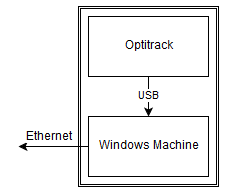
\includegraphics[scale=0.70]{verify_module.PNG}
\caption{Verification Module}
\label{fig:ver_mod}
\end{figure}

The Optitrack component relays its information back to the windows machine via USB, which then relays that information back to the control module via Ethernet.
\subsubsubsection{Verification Module Design}
\tab The design for this module was again rather simple, as the constraints of having to communicate through ROS and having to determine the location with complete accuracy only resulted in only one viable choice, the Optitrack system in the lab. This is because it is the only system able to accurately determine the location of the robot at any given moment and relay it back to the control module independently of the code running anywhere else in the system.

\subsection{Interface Descriptions}
\subsubsection{Software/Hardware Interface}
\tab As mentioned in the ROS section, the interface between the hardware and the software is facilitated through ROS. ROS allows the programmer to abstract away all of the communication details, and allows programmer to focus on a higher level of programming. The way ROS facilitates this communication is through the publisher-subscriber system. Certain nodes, or drivers, already exist in order to control the robot. These nodes wait for messages on the topic related to the hardware they control, and when they receive messages, they enact the controls necessary to carry out the command carried by the message. This makes the life of the programmer very easy, it removes the issue of dealing with interfacing to hardware, allowing the programmer to simply publish messages to the topics, and the driver nodes will take care of interacting with the hardware.

\subsubsection{Inter-Software Interfaces}
\tab The software also communicates via ROS’s publisher-subscriber system, which allows any process, or node, to subscribe to any number of topics and to publish to any number of topics. The details of this have already been described in the ROS section of this deliverable. Another way in which the software interacts is through function calls. Different modules have functions that can be called by other modules, which allows the programmer to decompose functions into logical groupings but still be able to access them from different modules.

\subsubsection{Control Module Interfaces}
\tab The control module has several interfaces. It interacts with the user via Linux I/O, which includes GUI-based programs as well as the terminal.  The control module interacts with the robot module via SSH. The robotics lab has an internal wifi network that is set up purely for this, to allow modules to interact wirelessly with others. Lastly, the control module receives updates from the verification module via Ethernet.

\subsubsection{Robot Module Interfaces}
\tab The robot module has four components. The central component, the laptop, interacts with the Kinect and with the base via USB. The base interacts with the internal sensors and actuators via internal signals. The robot module talks to the control module via SSH, as mentioned before. This is facilitated by the laptop, which has a wireless card and allows for SSH.

\subsubsection{Visualization Module Interfaces}
\tab The visualization module’s two components interact via USB, the windows machine being the component that receives data from the Optitrack via USB and then formats it and sends it via Ethernet to the control module.


\section{Equipment Identification}

\begin{figure}[h!]
\begin{center}
\begin{tabular}{| c | c | c |}
 \hline
 \textbf{Developed Items} & \textbf{Model/Part NO} & \textbf{Completion/Arrival Date} \\ 
 \hline
 Nil & Nil & Nil \\  
 \hline
 \textbf{Off-the-Shelf Items} & \textbf{Model/Part NO} & \textbf{Completion/Arrival Date} \\ 
 \hline
 Control Station &  & Available Day 0 in Lab \\  
 \hline
 Robot Computer &  & Available Day 0 in Lab \\
 \hline
 Turtlebot Base & IRobot Base & Available Day 0 in Lab \\
 \hline
 Kinect Sensor & Original Model & Available Day 0 in Lab \\ 
  \hline
 \textbf{Support Items} & \textbf{Model/Part NO} & \textbf{Completion/Arrival Date} \\ 
 \hline
 Optitrack &  & Available Day 0 in Lab \\  
 \hline
 Windows Machine &  & Available Day 0 in Lab \\
 \hline
 Brick-A-block &  & Arrived Mid-February \\
 \hline
\end{tabular}
\caption{Equipment Identification}
\label{fig:equipment_ID}
\end{center}
\end{figure}

\section{Testing and Results}
\subsection{Testing}
\tab Testing the project involved testing four different aspects. The first, and most fundamental aspect, was whether or not localization was achieved, and how long this process took. This was tested for both the normal re-sampling and the KLD re-sampling algorithms. The second aspect that was tested was whether or not the robot could regain the localization once it has been lost. This could happen due to many factors. The most common one is the kidnapped robot, where the robot would be picked up and moved to another spot. Another factor that could result in a localization being lost is that the original localization was off or wrong. This tends to happen in highly symmetric environments, where the robot may think that it is localized for a long time before realizing it isn't and needing to re-localize. The third aspect that was tested was the performance comparison between the normal re-sampling algorithm and the KLD re-sampling algorithm. This involved testing both the localization quality and time in different environments as well as testing the time-performance of these algorithms post-localization, meaning how well and how quickly they are able to track their locations once localized, which determined how well it could run alongside other tasks. The last aspect of the testing involved testing the fidelity of movement in the three directions($x, y, \theta$). The movement control is all done through ROS, so this simply involved issuing a movement command and testing how well the movement was executed using measuring tape.

\subsubsection{Testing for Localization}
\tab In order to test whether or not the algorithms could localize, each algorithm was ran 5 times, in two different environments, each time with different initial conditions (initial conditions being the initial position, $position = (x, y, \theta)$. The robot was considered localized once all of the particles converged to one cluster, and once the calculated position, or average of all particles, was within the limits specified by PR01 and PR02. The localization time was also measured in order to see if it was within the time specified by PR03. The first environment tested was a highly symmetric 4m by 4m room with different shapes at each edge. The map for this room can be seen in figure \ref{fig:square_room}. The environment was a less symmetric L-shaped room, the map for which can be seen in figure \ref{fig:l_room}. The first room, the square room, is designed to simulate a typical room-type environment, whereas the L-shaped room is designed to simulate a corridor-type environment. The results of these tests are outlined in the results section.

\begin{figure}[h!]
\centering
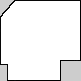
\includegraphics[scale=2.0]{roomImprovedTestAdv2.png}
\caption{Square Room Map}
\label{fig:square_room}
\end{figure}

\begin{figure}[h!]
\centering
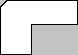
\includegraphics[scale=3.0]{Map.png}
\caption{L-Shaped Room Map}
\label{fig:l_room}
\end{figure}

\subsubsection{Testing for Re-Localizing After Getting Lost (Kidnapped Robot Problem)}
\tab In order to test whether or not the algorithms could solve the kidnapped robot problem, the robot was allowed to localize, then it was moved, and then it was seen if it could re-localize. Since solving this problem was not part of the initial requirements, there were no requirements to test against, instead, this was simply a completion test. If the robot was able to re-localize eventually (within 2 minutes of getting lost), it was considered a pass. However, if the robot was unable to re-localize within 2 minutes, it was considered a fail. The same environments were used for these tests. The maps for these environment can be seen in figures \ref{fig:square_room} and \ref{fig:l_room}.  

\subsubsection{KLD Sampling vs Normal Sampling}
\tab The last component of the project involved comparing two different re-sampling algorithms in particle filters, in order to determine which algorithm would be superior in which circumstances and to determine which algorithm would perform better once its localized and simply tracking its localization. In order to compare the two, the localization times were first compared to see the difference in the initial localization time. Then, once the algorithms were simply tracking the localization. The same environments were used for these tests, the loop times were compared to see how well these algorithms could perform when running alongside other tasks. The maps for these environment can be seen in figures \ref{fig:square_room} and \ref{fig:l_room}.  

\subsubsection{Testing for Fidelity of Movement}
\tab The project also involved robot movement, as as such it was necessary to ensure that the movement controls provided by ROS were accurate.In order to do this, the robot was placed at the start of a measuring tape and driven forward 10 times, each time measuring how far it moved. It was also ensured that the robot drove in a straight line, being no more than 10 degrees off of its intended line of movement. Lastly, turn commands were issued to ensure that the robot turned as desired.

\subsection{Results}
This section will describe the results obtained from the testing conducted for this project.

\subsubsection{Results of Localization Testing}
\tab The results of the localization testing demonstrated that both algorithms were able to localize in both environments every single time. However, the testing proved that neither algorithm was able to localize within the allotted 15 seconds, as stated by PR03. This is because both environments are too symmetrical, and because the robot's movement speed is too low. In order to properly localize, the robot needs to move around and test different hypotheses. The movement speed of the robot proved to be too low, so the robot was unable to collect enough data within the first 15-second window in order to localize correctly. The symmetry of the environments contributed to this because it meant that the robot needed to collect more data to localize, hence needed more time to move around. In general, it was found that placing a requirement on the amount of time needed to localize is completely unrealistic because depending on the environment, the localization process could require very few samples (in highly asymmetric environments), which would result in fast localization, or very many samples (highly symmetric environments), which results in slower localization. As such, a universal maximum localization time for all environments proved to be an unrealistic requirement. Figure \ref{fig:localization_times} shows the results for the localization tests. Figure /ref{fig:results-summary} outlines which requirements were met.

\begin{figure}[h!]
\centering
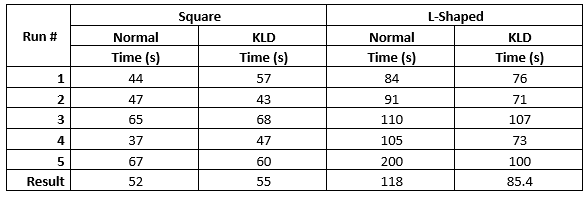
\includegraphics[scale=1.0]{Localization_Results.PNG}
\caption{Localization Results}
\label{fig:localization_times}
\end{figure}

\subsubsection{Kidnapped Robot Results}
\tab The results with regards to the kidnapped robot problem showed that the algorithm is robust enough to handle every case where the robot was localized and was then displaced. In both environments, the robot was displaced multiple times, each time eventually regaining it's localization and maintaining it well, until it was kidnapped again.

\subsubsection{Results of KLD vs Normal}
\tab The results of the localization testing demonstrated that both algorithms were able to localize in both environments every single time. However, the testing proved that normal re-sampling had a slightly lower localization time in the symmetric room, proving to be better for symmetric environments. This is because in KLD sampling, the particles are constantly re-sampled, and this proves to be dangerous in highly symmetric environments as  some estimates may be lost, with all the focus placed on one likely estimate, which in a symmetric environment is dangerous because it could mean that the wrong location for the localization is being focused on. In practice, this meant that the KLD algorithm was susceptible to catching a wrong localization, and then having to redistribute its particles and find itself again, resulting in slower localization times.\\

The results also showed that in less symmetric environments, such as the L-shaped room, KLD is the better algorithm. It was on average noticeably faster. While the normal algorithm performed marginally better in symmetric environments, the KLD algorithm proved far superior in less symmetric environments. What this result allows future programmers to do is to use the re-sampling algorithm that better suits their needs. For highly symmetric environments, such as rooms, it is better to use the normal re-sampling algorithm. However, in less symmetric environments, such as corridors, it is better to use KLD. An application for the room-type of environment would be a room cleaning robot, whereas an application for the corridor-type of environment would be a warehouse robot.\\

One comparison that was important to make between the two algorithms is the execution time of one loop, or one update. This is called the long-run performance, or how well the algorithm executes over time. This is important because localization algorithms usual run alongside other code, and therefor need to run quickly so that they don't eat up all the resources of the computer. In order to test this, the loops were timed twenty times for each algorithm, and averages were obtained. The normal re-sampling algorithm averaged a loop time of 1.21s, whereas the KLD re-sampling algorithm averaged a loop time of 0.86s. This means that on average, the normal re-sampling algorithm would take 40 present more time, meaning it uses up 40 percent more computational resources, which can become an issue if localization is ran alongside other CPU-intensive tasks. Please refer to figure \ref{fig:long-term} for the data used to calculate this.\\

\begin{figure}[h!]
\centering
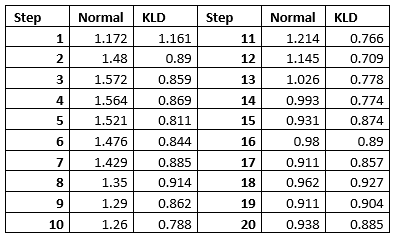
\includegraphics[scale=1.0]{long-run.PNG}
\caption{Single-Loop Execution Time Normal vs KLD}
\label{fig:long-term}
\end{figure}

\subsubsection{Results of Movement Testing}
\tab The movement testing proved that the control provided by ROS was more than sufficient for the requirements laid out by this project. The robot moved as expected each time, and despite having a wheel slip on several occasions, it was still within 10 degrees of its intended movement direction. The turn controls for the robot also proved that the robot was able to turn as desired, thereby demonstrating that the controls provided by ROS are more than sufficient for this project.

\subsubsection{Summary of Results}
\tab The testing results are summarized in figure \ref{fig:results_summary}. These results show that the majority of the requirements were met. The first one that was not met was FR03, which states that the robot shall be able to detect collisions using its bumper sensor. This requirement proved to be unnecessary however, as the autonomous driving algorithm already performed collision avoidance, meaning collisions would never occur. This requirement was therefor useless and was never implemented. The second requirement that was not fully met was FR05, this requirement was mostly met, however, the timing constraint, PR03, was broken. This has already been discussed in the previous sections, explaining why placing a timing requirement on an algorithm who's performance is entirely dependent on the environment its in is a terrible idea, and will always be broken given a complex enough environment. Overall, the project accomplished the stated goal of localization, and on top of that solved the kidnapped robot problem and explored different localization techniques to determine which techniques worked better in which environments. As such, the testing proved that our project was a success.

\begin{figure}[h!]
\centering
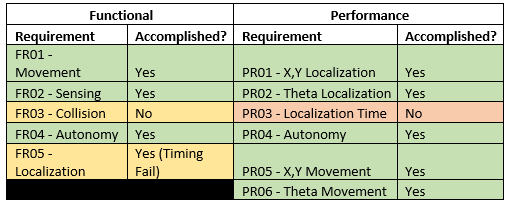
\includegraphics[scale=1.0]{Requirements-Summary.PNG}
\caption{Requirement Results Summary}
\label{fig:results_summary}
\end{figure}

\section{Summary}
\tab In order to solve the robot localization problem, an algorithm for MCL was written and implemented on the Turtlebot robot platform. MCL is an algorithm for localization that samples random locations on a map of the environment, and compares what should be detected by the robot's sensors at those locations to what is actually being sensed by the robot. The sample locations, known as particles, are then redistributed such that they cluster at the probable locations of the robot, ultimately all collapsing to the robot's true location.\\

The Turtlebot was chosen to implement this algorithm as it has all the actuators necessary for localization and uses ROS, a software package which allowed the abstraction away trivial problems such as driving the motors and interfacing with the camera. Since localization is most often run alongside another primary task, three different methods of moving the Turtlebot were used while testing the localization algorithm. The first had the Turtlebot move via remote control from a computer and keyboard giving wireless commands to the Turtlebot computer. The second method of movement was autonomous, having the Turtlebot simply drive, avoid obstacles, and localize. The final way in which the robot was driven was tracking a target. This was done using a laser pointer which the robot turns to face, and drives towards if it will not hit an obstacle.\\

Redistributing the particles can be done in different ways. For this project, two methods of particle redistribution known as normal distribution and KLD were tested and compared. The normal method redistributes the same number of particles each iteration of the loop, whereas KLD lowers the amount of particles needed as the particles cluster. This lowers the processing time required for each iteration. In our results we found that, as predicted, KLD generally caused the robot the localize quicker. However, KLD struggled more with highly symmetrical environments as it was often incorrectly eliminating particles that still held merit.\\

It was found across both methods of particle distribution, and across the movement functions, that the robot could not only localize autonomously, but could effectively localize again when it was subject to the Kidnapped Robot Problem. This demonstrated that the MCL algorithm was both effective and robust.\\

One last generic result that can be drawn from the testing is related to the use of a linear approximation for the calculation of the KL-bound. The paper outlining the KL-bound presented it as a complex calculation involving square roots and exponentiation, both computationally-intensive processes. It was demonstrated in this paper that a linear approximation could be used with equally good results, and that for future work programmers should strive to use a linear approximation when using KLD re-sampling in order to save some processing power.

\section{Conclusion}
\tab Every project has an intended purpose, and this one was no different. The purpose of this project was to solve the localization problem while comparing different methods in order to see which one works best. The results demonstrated that the localization problem can be solved very well using particle filtering, which allows for not only regular localization, but for also easily solving the kidnapped robot problem. Our results therefor demonstrate that particle filtering is a viable solution to this problem.\\

Additionally, our results demonstrate that the particle filter solution to the localization problem can be further optimized by matching the re-sampling algorithm to the environment in which the robot is working. This provides future programmers with the ability to optimize their localization performance. If the robot is running in a room-type environment, a highly symmetrical environment, then normal sampling proved to be superior. In corridor-type environments, KLD sampling proved better. Future programmers refer to these results, saving them the work of having to figure out which localization algorithm to use in their particlar case.\\

When deciding to use ROS, we chose to use it because it is an open-source software where problems that have been solved in the past such as movement and sensing can be ignored, and new problems can be explored. This means that ROS allows for researchers and programmers alike to build on the work of others in order to not waste time with mundane tasks and explore new problems. We believe, and truly hope that the work done in this project will allow future users of ROS to better determine which localization algorithms they need for the problems that they are exploring and focus on much more complex problems, thereby promoting the ROS spirit of not having to solving problems that have already been explored.

\section{Discussion}\label{fig:disc}
\tab While the desired outcome for the project was achieved, the progression of the project passed quite differently than expected. Understanding localization and the MCL algorithm turned out to be an exercise in itself. To properly equip ourselves for developing the algorithm in C++ for the Turtlebot, we first wrote simulations in MATLAB building up to the final product. The first simulation was an implementation of MCL in just one dimension, a robot moved linearly along a line and the particles clustered around it and other landmarks whenever it passed a marked position on the line. When this simulation was working, we moved on to a two-dimensional MATLAB simulation. This looked closer to the final product as the particles and the robot were marked with X and Y components, however they did not yet have a direction in this simulation. Instead landmarks were placed at random points in the 2D space and the weights were assigned to each particle based on its proximity to its closest landmark. Only after we finished these simulations did we attempt to code the same algorithm in ROS.\\

ROS, however, presented a whole new set of challenges. Alongside writing simulations for the algorithm, we worked our way through ROS tutorials online to better understand the structures involved with the software. ROS is not designed to be user friendly, but it is an extremely powerful tool for programming robotics. Its publisher-subscriber model made it easy to test different movement functions with different methods of particle redistribution. Before tackling a project such as this we believe it is necessary to have a strong understanding of ROS, and studying the software platform should always be a priority before facing the problem.\\

We had not initially planned on including a movement module for objective tracking. This was an addition to the project adapted from software we had seen implemented on the Turtlebot before, which would turn the robot to face a laser pointer\citep{Tracker}. We adapted this software to be useful for our project and ran it alongside our localization script because it is a perfect example of localization taking place alongside another primary task. Localization is a difficult problem, but a robot that can localize itself and do nothing else is of no use to anyone. This is why we felt it was important to test it while accomplishing an actual goal. Autonomous movement is still responsible for the data used in the results. The implementation of the objective tracker was simply to prove that it could be done within our model, and that the algorithm used was effective and realistic.\\

Another important piece of information we learned throughout development was that localization struggles heavily in symmetrical spaces. A robot cannot possibly localize itself in a perfectly square room, because there are always four directions it could be facing with no way of distinguishing them. While we didn't test our robot in a perfectly symmetrical environment, we do suspect that symmetry is responsible for some of the longer localization times. Particularly in the environment where the walls are all the same and only the corners have unique properties, this is believed to have slowed the robot down. It needed to reach a corner before it could gather useful data. However, this was a good environment model for testing in as it is important to test the robot under demanding conditions. A robot that can localize well in a near symmetrical environment will localize great in a more unique environment. With more time to perform the tests we would have loved to have tested the robot across a wider range of environments to prove this claim, and to present better average localization times for the robot.\\

It was briefly discussed in section \ref{fig:autom} that the robots blind spots could be removed, or at least made smaller, with a wider scan angle. However this is not the only reason a wider scan angle should be considered. If the robot was to use a sensor that could take a full 360 degree laser scan it would have six times as much data at each point, which we believe would allow it to localize more effectively. It is important to note here, that updating the particles at each point would also take six times as long, assuming the scan uses the same number of range returns per degree, so this is not how this method would save time. Time would be saved because for every six moves our robot makes, a robot with a 360 degree laser scan would only need to make one whilee spending the same amount of time on computation. It would also localize more quickly because in the full-circle scan's first return, all of the data is new and this complementary data that will quickly narrow down the results. Our robot's scans do not always complement each other since the robot is often reading information about its position that provides the same information as a previous return, so the first six scans of the Turtlebot will never be as useful as the first scan of a robot performing a full circle scan.\\

All these factors considered, the MCL algorithm implemented on the Turtlebot still exceeded all the project requirements except one. When we initially developed our project environment we estimated an ability to localize within 15 seconds, thinking this would be more than sufficient. This is extremely unrealistic given the movement speed of the Turtlebot, and because in our final realization of the algorithm the robot must stop moving each iteration while it performs the calculations for the movement and measurement updates. The constant starting and stopping slows down the movement process significantly, but it is a necessity as the calculations for one iteration of the algorithm take longer than the motion of the physical robot. A possible fix for this would be to have the robot move at a constant, albeit much lower, speed that has the robot reach its destination each loop as the particle redistribution finishes. This problem itself would be nontrivial, as the time it takes the robot to perform one iteration of the algorithm varies circumstantially and with the amount of particles being used, and so such a solution was outside the scope of our project. Despite not meeting this design requirement, we still consider our final product to have successfully achieved our aim of robot localization.\\

\section{Future Work}
\tab Throughout the implementation of the localization algorithm, a number of options were compared while trying to produce the best results. For example, comparing different methods of particle redistribution found situations in which algorithms produced the more rapid and accurate results. However, there are other components of the project that were not explored as deeply due to time constraints, and could possibly be changed for better results.\\

\subsection{Extended Kalman Filter}
\tab A significant change that could be implemented to this project would be to localize using an Extended Kalman Filter(EKF) instead of Monte Carlo Localization. While Monte Carlo localization can still be found in certain products, EKF is more prevalent and used in a wide variety of systems, including GPS, for localization.\\

\begin{figure}[h!]
\centering
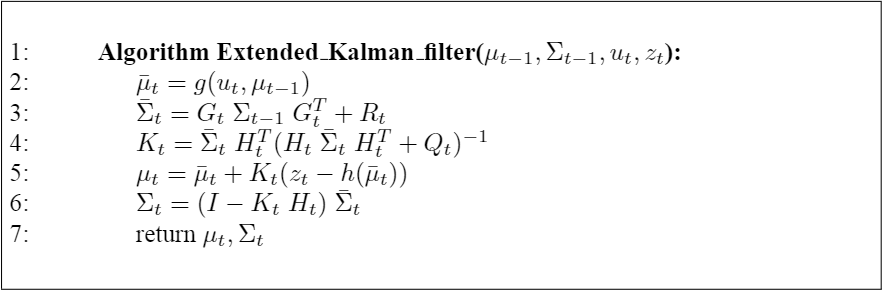
\includegraphics[scale=0.45]{ekf_algorithm.PNG}
\caption{The Extended Kalman Filter (EKF) Algorithm}
\label{fig:ekf}
\end{figure}

As shown in figure \ref{fig:ekf}, EKF works off of an entirely different algorithm than Monte Carlo. Using this method of localization, the particle filtering used during Monte Carlo would be irrelevant. Therefore, when exploring the possibility of EKF localization, it is recommended that the hardware architecture be the same structure as was used in this project's implementation on the Turtlebot. However, the software would need to be entirely different, while still being run in a ROS environment.\\

\subsection{Further Possibilities For Particle Redistribution}
\tab A significant factor in optimizing the robots ability to localize was the comparing of different methods for redistributing the particles. While both the normal distribution and KLD algorithms were tested for this, more certainly exist and the amount of methods that could be tested in this project was limited by time constraints. It is possible that an algorithm for particle redistribution that could more effectively localize the robot exists and it was simply not explored in this project. A possibility for future work would be taking this product as is and varying the particle redistribution algorithm among a larger group of solutions, to find the one the produces the best results.\\

Furthermore, the distribution methods that were implemented during this project, normal and KLD, were tested in two environments for five iterations each. While the data gathered is sufficient to support the conclusions drawn about the two algorithms, there is certainly more room for each of them to be explored further. One way to gather more data on these algorithms is vary the amount of particles used in each, and compare how this changes the localization times. More particles mean higher likelihood that particles will be found at the exact location of the robot, but it also means longer processing time between movements. Another way to explore these methods of distribution would be to test them across a wider range of environments. The two environments used in the tests were of reasonable size for the Turtlebot. A more thorough study of this project would involve testing it in very large and very small environments, and exploring if and how this causes the particle distribution to struggle. These are situations that would have been explored more had there been more time to test the final project.\\

\subsection{Better Pathing and Movement Updates}\label{fig:fwpathing}
\tab This project never called for any sort of pathing or optimized movement. Having the robot explore with room systemically was more than sufficient to prove its ability to localize. However, it is obvious that there exist better motion processes for focusing on localization. One possible exercise with this product would be to design an autonomous movement component more intelligent than the three used in this project. One such design could be to make the robot towards a point where it would see a unique landmark if its most probable cluster of particles was correct. This idea for smart movement pathing would almost certainly lower the amount of iterations required to localize the robot. This ability to make movement decisions autonomously is very similar to what the user imposes on the robot when attempting to localize via remote control, driving the robot towards distinguishing landmarks. This exercise almost always allows the robot to localize itself in fewer steps. However, as the focus was a working localization algorithm, intelligent movement was certainly outside the scope of this project.\\

It is worth noting, however, that designing a robot to move systemically for localization is irrelevant to the functionality of the algorithm. As was described earlier, localization is always implemented alongside another primary task as a robot that is capable only of localization serves no practical purpose. Since the movement requirements of the primary task will likely subsume the optimal movement for localization, the localization algorithm must be effective whether or not the motion function is making optimal decisions.\\

It was briefly discussed in section \ref{fig:disc} that a possibility for lowering the time required to localize would be to have the robot move continuously, rather than stopping to perform calculations each loop. This would speed up the localization process as the robot would not be constantly needing to accelerate while it is trying to localize. However, the only way in which this can be attained while maintaining the current implementation of MCL would be to have to robot move at a much slower speed that has it reaching its destination and completing its current loop simultaneously. This would mean the robot would perform its calculations while moving. Processing time varies with particle distribution method, amount of particles being used, range returns from the scan angle, and computer processing ability. This makes it very hard to match the rate of two different loops. Clearly, a movement component this intricate was outside the scope of this project, however it would be an interesting exercise to explore in the future.

\begin{appendices}
\section{Monte Carlo Localization Code for Turtlebot}\label{fig:mclcode}.
\subsection{Localization.h}
\begin{lstlisting}[language=C++]
/*
 * Localization.h
 *
 * This module contains all of the information necessary for localization
 *
 *  Created on: Feb 4, 2017
 *      Author: Michael Kogan and Garrett McDonald
 */

#ifndef LOCALIZATION_H_
#define LOCALIZATION_H_

#include "ros/ros.h"
#include "std_msgs/String.h"
#include "sensor_msgs/LaserScan.h"
#include "nav_msgs/OccupancyGrid.h"
#include "nav_msgs/MapMetaData.h"
#include "geometry_msgs/PoseStamped.h"
#include "geometry_msgs/PoseArray.h"
#include "geometry_msgs/Quaternion.h"
#include "geometry_msgs/Twist.h"
#include <sstream>
#include <iostream>
#include <stdio.h>
#include <math.h>
#include <vector>
#include <time.h>
#include <stdlib.h>

#define PI 3.14159265
#define ONE_OVER_SQRT_2PI 0.3989422804
#define MIN_RANGE 0.45
#define MAX_RANGE 4.0
#define MAX_RETRIES 5
#define ANG_DT 0.4
#define LIN_DT 0.5
#define X_CONVERGE 0.35
#define Y_CONVERGE 0.35
#define THETA_CONVERGE 10
#define MIN_PARTICLES 500
#define PARTICLE_LIMIT 1000
#define Z_099 0.83891
#define EPSILON 0.05
#define BIN_LENGTH 0.5
#define BIN_ANGLE 10



using namespace std;

/**
 * Structure used to keep track of the position:
 * 	x -> The x coordinate
 * 	y -> The y coordinate
 * 	theta -> The angle which the position is facing
 */
struct pose{
	float x;
	float y;
	float theta;
};

/**
 * Structure used to keep track of the map:
 * 	map -> The occupancy grid
 * 	width -> The width
 * 	height -> The height
 *      resolution -> The resolution
 */
struct mapStruct{
	signed char **map;
	int width;
	int height;
	float resolution; 
};

/**
 * Structure used to represent a particle:
 * 	position -> The location of the particle
 * 	weight -> The weight associated with the particle
 */
struct particle{
 pose position;
 double weight;
};

/**
 * This type will allow us to point different functions to a generic localization function
 */
typedef vector<particle> (*RESAMPLING_FUNCTION) (vector<particle>, vector<double>);

/**
 * This function normalizes the given angle
 *
 * @param
 * 	angle -> The angle that we are normalizing
 * @return
 * 	float -> The normalized angle
 */
float normalizeAngle(float angle);

/**
 * This function calculates the distance given a dx, dy, and a theta
 *
 * @param
 * 	dx -> The x displacement
 * 	dy -> The y displacement
 * 	theta -> The angle at which we are looking
 * @return
 * 	float -> The distance
 */
float calculateDistance(int dx, int dy, float theta);

/**
 * This function projects the values of a range scan performed by the robot
 *
 * @param
 * 	p -> The position of the robot on the map
 * 	resolution -> The resolution of the map in cm
 * 	angleCount -> The amount of angles that we wish to generate (suggested is 61, to scan +- 30 degrees from direction in pose
 * 	minRange -> The minimum range of the sensor
 * 	maxRange -> The maximum range of the sensor
 * @return
 * 	vector<float> -> A vector the size of angleCount containing the projected distance values
 */
vector<float> generateView(pose p, float resolution, int angleCount, float startAngle, float angleResolution);
/**
 * This function generates a map given a set of points, a height, and a width, setting it to the global variable
 *
 * @param
 * 	points -> The set of points in row-ordinal form
 * 	h -> The height of the map
 * 	w -> The width of the map
 *      r -> The resolution of the map
 */
void generateMap(signed char points[], int h, int w, float r);

/**
 * This function gives the normal probability of result actual given a mean and a standard deviation
 *
 * @param
 * 	actual -> The result
 * 	mean -> The mean of the distribution
 * 	std_dev -> The standard deviation of the distribution
 * @return
 * 	float -> The probability of result actual in the distribution
 */
double normalPDF(float actual, float mean, float std_dev);

/**
 * This function determines the weight of an estimate using the projected view and the actual view
 *
 * @param
 * 	scan -> The reading that we measured from the environment
 * 	loc -> The location at which we believe we are at
 * @return
 * 	float -> The relative weight based on how likely our measurement is given our position
 */
double measurementModel(sensor_msgs::LaserScan scan, pose loc);

/**
 * This function applies the movement as defined by the linear and angular velocity, adding some variation to simulate the noise of the system
 *
 * @param
 * 	prevLoc -> The starting location
 * 	v -> The linear velocity
 * 	w -> The angular velocity
 * 	dt -> The amount of time for which we are applying the angular/linear velocities
 * @return
 * 	pose -> The new location after applying the movement
 */
pose movementModel(pose prevLoc, float v, float w);

/**
 * This function draws a sample from a normal distribution given variance b
 *
 * @param
 *  b -> The variance of the normal distribution
 * @return
 *  float -> The sample
 */
double sample(float b);

/**
 * This function takes the array from a /scan message and converts it to a 61-sized array (ANGLE_COUNT)
 *
 * @param
 * 	scan -> The raw data from the /scan message
 * @return
 * 	vector<float> -> The processed data, a 61-sized array of measurements
 */
vector<float> convertScan(vector<float> scan, int size);

/**
 * This function returns the map as a mapStruct
 *
 * @return
 * 	mapStruct -> The map and pertinent metadata
 */
mapStruct getMap(void);

/**
 * This function creates and distributes the number of particles specified by the NUM_PARTICLES constant
 *
 * @return
 * 	vector<particle> -> The list of particles
 */
vector<particle> distributeParticles(void);

/**
 * This function generates a random float specified by the boundaries
 *
 * @param
 * 	min -> The min value
 *	max -> The max value
 * @return
 * 	float -> The random value
 */
float generateRandomFloatBetween(float min, float max);

/**
 * This function generates a random double specified by the boundaries
 *
 * @param
 * 	min -> The min value
 *	max -> The max value
 * @return
 * 	float -> The random value
 */
double generateRandomDoubleBetween(double min, double max);

/**
 * This function will display the particles and the position of the robot
 *
 * @param
 *	particles -> The particles with which we are working
 *	ros::Publisher -> The publisher object for the particles
 *	ros::Publisher -> The publisher object for the position
 */
void displayResults(vector<particle> particles, ros::Publisher par, ros::Publisher pose);

/**
 * This function will generate a random position on the map
 *
 * @return
 *	pose -> The random position on the map
 */
pose generateRandomPositionOnMap();

/**
 * This function performs a basic uniform resampling of the particles
 *
 * @param
 *	particles -> The particles with which we are working
 *	cumsum -> The cumulative sum
 * @return
 *	vector<particles> -> The resamples particles
 */
vector<particle> uniformResample(vector<particle> particles, vector<double> cumsum);

/**
 * This function performs KLD resampling of the particles
 *
 * @param
 *	particles -> The particles with which we are working
 *	cumsum -> The cumulative sum
 * @return
 *	vector<particles> -> The resamples particles
 */
vector<particle> kldResample(vector<particle> particles, vector<double> cumsum);

/**
 * This function will return the number of particles
 *
 * @return
 *	int -> The total number of particles
 */
int getNumParticles(void);

#endif /* LOCALIZATION_H_ */

\end{lstlisting}

\subsection{Localization.cpp}
\begin{lstlisting}[language=C++]
/*
 * Localization.cpp
 *
 * This module contains the implementations of the functions in Localization.h
 *
 *  Created on: Feb 4, 2017
 *      Author: Michael Kogan and Garrett McDonald
 */

#include "Localization.h"

signed char **myMap;
int height, width, seqID = -1, noParticles = 1000;
float resolution;

float normalizeAngle(float angle){
	float rtn = angle;
	while(rtn < 0)
		rtn += 2*PI;
	while(rtn > 2*PI)
		rtn -= 2*PI;
	return rtn;
}

float calculateDistance(int dx, int dy, float theta){
	if ((theta > PI / 4 && theta < 3 * PI / 4)
				|| (theta > 5 * PI / 4 && theta < 7 * PI / 4))
		return abs(dx/sin(theta))*resolution;
	return abs(dy/cos(theta))*resolution;
}

vector<float> generateView(pose p, float resolution, int angleCount, float startAngle, float angleResolution) {
	vector<float> scan(angleCount);
	float x = p.x, y = p.y, theta = 2*PI - p.theta;
	int startX = y / resolution, startY = x / resolution;
	for (int i = 0; i < angleCount; i++) {
		float offset, currentAngle = normalizeAngle(theta - i * angleResolution + startAngle),
				runningOffset = 0, directionX = sin(currentAngle), directionY =
						cos(currentAngle);
		int dx = 0, dy = 0;
		if ((currentAngle > PI / 4 && currentAngle < 3 * PI / 4)
				|| (currentAngle > 5 * PI / 4 && currentAngle < 7 * PI / 4)) {
			offset = fabs(1 / tan(currentAngle));
			while (myMap[startX + dx][startY + dy] == 0
					&& calculateDistance(dx, dy, currentAngle) < MAX_RANGE) {
				if (directionX > 0)
					dx--;
				else
					dx++;
				if (directionY > 0)
					runningOffset += offset;
				else
					runningOffset -= offset;
				dy = round(runningOffset);
			}
		} else {
			offset = fabs(tan(currentAngle));
			while (myMap[startX + dx][startY + dy] == 0
					&& calculateDistance(dx, dy, currentAngle) < MAX_RANGE) {
				if (directionX > 0)
					runningOffset -= offset;
				else
					runningOffset += offset;
				if (directionY > 0)
					dy++;
				else
					dy--;
				dx = round(runningOffset);
			}
		}
		float range = calculateDistance(dx, dy, currentAngle);
		if(range < MIN_RANGE || range > MAX_RANGE)
			range = MAX_RANGE;
		scan[i] = range;
	}
	return scan;
}

void generateMap(signed char points[], int h, int w, float r){
	myMap = 0, height = h, width = w, resolution = r;
	myMap = new signed char*[height];
	for(int i = 0; i < height; i++){
		myMap[i] = new signed char[width];
		for(int j = 0; j < width; j++){
			myMap[i][j] = points[i*width+j];
		}
	}
}

double normalPDF(float actual, float mean, float std_dev){
	double pow = (actual-mean)/std_dev;
	return ONE_OVER_SQRT_2PI/std_dev*exp(-0.5*pow*pow);
}

double measurementModel(sensor_msgs::LaserScan scan, pose loc){
	int angleCount = (scan.angle_max - scan.angle_min)/scan.angle_increment;
	vector<float> projected = generateView(loc, resolution, angleCount, scan.angle_max, scan.angle_increment), measured = convertScan(scan.ranges, angleCount);
	float w = 1, p;	
	for(int i = 0; i < angleCount; i++){
		p = 0;
		if(measured[i] == MAX_RANGE)
			p += 0.05;
		p += (normalPDF(measured[i], projected[i], 3*resolution)/normalPDF(projected[i], projected[i], 3*resolution))*0.95;
		w+=p;
	}
	return w;
}

pose movementModel(pose prevLoc, float v, float w){
	float v_prime = v + sample(0.3*v + 0.3*w), w_prime = w + sample(0.3*v+0.3*w), gamma = sample(0.05*v+0.05*w), divisor = v_prime/w_prime;
	float x = prevLoc.x - divisor*sin(prevLoc.theta) + divisor*sin(prevLoc.theta + w_prime*LIN_DT);
	float y = prevLoc.y + divisor*cos(prevLoc.theta) - divisor*cos(prevLoc.theta + w_prime*LIN_DT);
	float theta = normalizeAngle(prevLoc.theta + w_prime*ANG_DT + gamma*ANG_DT);
	int dx = round(x/resolution);
	int dy = round(y/resolution);
	if(dx >= width || dy >= height || dx < 0 || dy < 0){
		return generateRandomPositionOnMap();
	}	
	int noRetries = 0;
	while(myMap[dy][dx] != 0){
		if(noRetries == MAX_RETRIES){
			return generateRandomPositionOnMap();
		} else {
			x = prevLoc.x - divisor*sin(prevLoc.theta) + divisor*sin(prevLoc.theta + w_prime*LIN_DT);
			y = prevLoc.y + divisor*cos(prevLoc.theta) - divisor*cos(prevLoc.theta + w_prime*LIN_DT);
			dx = round(x/resolution);
			dy = round(y/resolution);
			noRetries++;
		}
	}
	pose nPose;
	nPose.x = x;
	nPose.y = y;
	nPose.theta = theta;
	return nPose;
}

double sample(float b){
	double s = 0;
	for(int i = 0; i < 12; i++){
		s += generateRandomDoubleBetween(-1,1);
	}
	return b/6*s;
}

vector<float> convertScan(vector<float> scan, int size){
	vector<float> parsed(size);
	for(int i = 0; i < size; i++){
		if(isnan(scan[i]) || scan[i] > MAX_RANGE)
			parsed[i] = MAX_RANGE;
		else
			parsed[i] = scan[i];
	}
	return parsed;
}

mapStruct getMap(){
  mapStruct m;
  m.map = myMap;
  m.height = height;
  m.width = width;
  m.resolution = resolution;
  return m;
}

vector<particle> distributeParticles(){
	vector<particle> particles = vector<particle>(noParticles);
	for(int i = 0; i < noParticles; i++){
		particle par;
		par.position = generateRandomPositionOnMap();
		par.weight = 1/noParticles;
		particles[i] = par;
	}
	return particles;
}

float generateRandomFloatBetween(float min, float max){
	return min + static_cast <float> ((rand()))/(static_cast <float> (RAND_MAX/(max-min)));
}

double generateRandomDoubleBetween(double min, double max){
	return min + static_cast <double> ((rand()))/(static_cast <double> (RAND_MAX/(max-min)));
}

void displayResults(vector<particle> particles, ros::Publisher par, ros::Publisher pose){
	float x = 0, y = 0, theta = 0;	
	seqID++;
	geometry_msgs::PoseArray parts;
	geometry_msgs::PoseStamped position;
	parts.header.seq = (unsigned int)seqID;
	parts.header.stamp = ros::Time::now();
	parts.header.frame_id = "/map";
	position.header.seq = (unsigned int) seqID;
	position.header.stamp = ros::Time::now();
	position.header.frame_id = "/map";
	for(int i = 0; i < noParticles; i++){
		geometry_msgs::Pose p;
		geometry_msgs::Quaternion quat;
		p.position.x = particles[i].position.x;
		p.position.y = particles[i].position.y;
		p.position.z = 0;
		quat.w = std::cos(particles[i].position.theta*0.5);
		quat.x = 0;
		quat.y = 0;
		quat.z = std::sin(particles[i].position.theta*0.5);
		p.orientation = quat;
		parts.poses.push_back(p);	
		x += particles[i].position.x;
		y += particles[i].position.y;
		theta += particles[i].position.theta;	
	}
	position.pose.position.x = x/noParticles;
	position.pose.position.y = y/noParticles;
	position.pose.position.z = 0;
	theta /= noParticles;
	position.pose.orientation.w = std::cos(theta*0.5);
	position.pose.orientation.x = 0;
	position.pose.orientation.y = 0;
	position.pose.orientation.z = std::sin(theta*0.5);
	par.publish(parts);
	pose.publish(position);
}

pose generateRandomPositionOnMap(){
	pose pos;
	pos.x = generateRandomFloatBetween(0.0, (width-1)*resolution);
	pos.y = generateRandomFloatBetween(0.0, (height-1)*resolution);
	pos.theta = generateRandomFloatBetween(0.0, 2*PI);
	int dx = round(pos.x/resolution);
	int dy = round(pos.y/resolution);
	while(myMap[dy][dx] != 0){
		pos.x = generateRandomFloatBetween(0.0, (width-1)*resolution);
		pos.y = generateRandomFloatBetween(0.0, (height-1)*resolution);	
		dx = round(pos.x/resolution);
		dy = round(pos.y/resolution);
	}
	return pos;	
}

vector<particle> uniformResample(vector<particle> particles, vector<double> cumsum){
	vector<particle> newParticles = vector<particle>(noParticles);
	for(int i = 0; i < noParticles; i++){
		double guess = generateRandomDoubleBetween(0.0,1.0);
		int j = 0;
		while(cumsum[j] < guess){
			j++;			
		}
		particle p;
		p.position = particles[j].position;
		p.weight = 0;
		newParticles[i] = p;
	}
	return newParticles;
}

vector<particle> kldResample(vector<particle> particles, vector<double> cumsum){
	vector<particle> newParticles = vector<particle>();
	int newNoParticles = 0, kldBound = MIN_PARTICLES, noBins = 0;
	bool bins[(int)(height*resolution/BIN_LENGTH + 1)][(int)(width*resolution/BIN_LENGTH + 1)][(int)(360/BIN_ANGLE)];
	do{
		double guess = generateRandomDoubleBetween(0.0,1.0);
		int j = 0;
		while(cumsum[j] < guess){
			j++;			
		}
		particle p;
		p.position = particles[j].position;
		p.weight = 0;
		newParticles.push_back(p);	
		int x = p.position.y/BIN_LENGTH, y = p.position.x/BIN_LENGTH, theta = ((2.0*PI - p.position.theta)*180.0/PI)/BIN_ANGLE; 
		if(bins[x][y][theta] == false){
			noBins++;
			bins[x][y][theta] = true;	
		}
		if(newNoParticles >= MIN_PARTICLES - 2 && noBins > 1){
				kldBound = ((noBins - 1)/(2*EPSILON))*pow((1-2/(9*(noBins-1))+sqrt(2/(9*	(noBins-1)))*Z_099),3);
		}	
		newNoParticles++;
	}while((newNoParticles < MIN_PARTICLES || newNoParticles < kldBound) && newNoParticles < PARTICLE_LIMIT);
	noParticles = newNoParticles;
	cout<<"KLD: " << ((noBins - 1)/(2*EPSILON))*pow((1-2/(9*(noBins-1))+sqrt(2/(9*(noBins-1)))*Z_099),3) <<"\n";
	cout<<"Bins: " << noBins << "\n";
	cout<<"New num particles: " << noParticles << "\n";
	return newParticles;
}

int getNumParticles(){
	return noParticles;
}
\end{lstlisting}

\subsection{Main.cpp}
\begin{lstlisting}[language=C++]
/*
 * main.cpp
 *
 * This module contains the main function running the MCL algorithm
 *
 *  Created on: Feb 4, 2017
 *      Author: Michael Kogan and Garrett McDonald
 */

#include "Localization.h"

/**
 * This is the main function
 *
 * @param 
 * 	argc -> The number of arguments
 *	argv -> The arguments
 *
 * @return
 * 	0 -> Success
 * 	Others -> Error codes
 */
int main(int argc, char **argv)
{
	RESAMPLING_FUNCTION resample;
	//Get argument
	if(argc != 2){
		cout << "Usage: mcl <resampling algorithm number>\n";
		cout << "0: Normal resampling\n";
		cout << "1: KLD resampling\n";
		return 0;
	}
	char resamplingAlgoNumber = *(argv[1]) - 48;
	switch(resamplingAlgoNumber){
		case 0:
			cout<<"Normal Resampling\n";
			resample = &uniformResample;	
			break;
		case 1:
			cout <<"KLD Resampling\n";
			resample = &kldResample;
			break;
		default:
			cout << "Usage: mcl <resampling algorithm number>\n";
			cout << "0: Normal resampling\n";
			cout << "1: KLD resampling\n";
			return 0;
	}
	//Random seed
	srand((unsigned int)time(NULL));

	//Initialize the node, declare a node handle
	ROS_INFO("Initializing node \"mcl\"");	
  	ros::init(argc, argv, "mcl");
  	ros::NodeHandle n;

	//We will be publishing the particles as a pose array
	ros::Publisher particlePub = n.advertise<geometry_msgs::PoseArray>("/particles", 100);

	//We will be publishing the location as a pose
	ros::Publisher posePub = n.advertise<geometry_msgs::PoseStamped>("/position", 100);

	//Used to synchronize with teleop
	std_msgs::String s;
	ros::Publisher synch = n.advertise<std_msgs::String>("/Synch", 100);
  
 	//Read in map
	ROS_INFO("Getting map from topic \"/map\"");
 	nav_msgs::OccupancyGrid map = *(ros::topic::waitForMessage<nav_msgs::OccupancyGrid>("/map", n));
 	generateMap(&map.data[0], map.info.height, map.info.width, map.info.resolution);

	//Distribute Particles
	ROS_INFO("Distributing particles");
	vector<particle> particles = distributeParticles();

	//Keep running node while ROS is good to go
 	while (ros::ok())
 	{	
		//Get next movement update
		geometry_msgs::Twist move = *(ros::topic::waitForMessage<geometry_msgs::Twist>("cmd_vel_mux/input/teleop", n));

		//Apply movement update to aprticles while waiting for robot to finish moving
		for(int i = 0; i < getNumParticles(); i++){
			particles[i].position = movementModel(particles[i].position, move.linear.x, move.angular.z);
		}
	
		//If min number of particles, allow move to finish
		if(getNumParticles() == 500){
			ros::Duration(0.25).sleep();		
		}

 		//Get Sensor Update
		sensor_msgs::LaserScan scan = *(ros::topic::waitForMessage<sensor_msgs::LaserScan>("/scan", n));
		
		//Normalization factor
		double normFac = 0;

		//Apply motion update and recalculate weights based on sensor update, and calculate the normalization factor
		for(int i = 0; i < getNumParticles(); i++){
			particles[i].weight = measurementModel(scan, particles[i].position); 
			normFac+=particles[i].weight;
		}
		
		//If nothing matches, redistribute
		if(normFac <= 50*getNumParticles()){
			particles = distributeParticles();
			synch.publish(s);
			continue;
		}

		ROS_INFO("NORMFAC: %f", normFac);

		//Create CDF
		vector<double> cumsum = vector<double>(getNumParticles());
		cumsum[0] = particles[0].weight;		
		for(int i = 1; i < getNumParticles(); i++){
			cumsum[i] = (cumsum[i-1] + particles[i].weight);	
		}
		
		for(int i = 0; i < getNumParticles(); i++){
			cumsum[i]/=normFac;
		}

		//Resample particles
		particles = resample(particles, cumsum);
		
		//Display Results in RViz
		displayResults(particles, particlePub, posePub);
		
		//Send synch message	
		synch.publish(s);
  	}
  	return 0;
}
\end{lstlisting}

\section{Teleop Code}
\subsection{mclTeleop.h}
\begin{lstlisting}[language=C++]
/*
 * mclTeleop.h
 *
 * This module contains all of the information necessary for the mclTeleop ROS Package
 *
 * 	Created on 11 March 2017
 *		Authors: Garrett McDonald and Michael Kogan
 */

#include "stdio.h"
#include "stdlib.h"
#include <termios.h>          
#include <unistd.h> 
#include "ros/ros.h"
#include "geometry_msgs/Twist.h"
#include "std_msgs/String.h"

#define LIN_VEL 0.25
#define ANG_VEL 0.218

/**
 * This function will swap out the console to one that has no console echo or buffering
 */
void swapConsole(void);

/**
 * This function will restore the original console
 */
void restoreConsole(void);
\end{lstlisting}

\subsection{main.cpp}
\begin{lstlisting}[language=C++]
/*
 * main.cpp
 *
 * This is the main module for the mclTeleop ROS package
 *
 * @param
 *	argc -> The number of arguments
 * 	argv -> The arguments
 *
 * @return
 *	0 -> Success
 *	Others -> Error codes
 *
 * 	Created on 11 March 2017
 *		Authors: Garrett McDonald and Michael Kogan
 */
#include "mclTeleop.h"

int main(int argc, char **argv){
	//Initialize node
	ros::init(argc, argv, "mclTeleop");
	//Create node handle
  	ros::NodeHandle n;
	//Advertise the topic
	ros::Publisher velocity = n.advertise<geometry_msgs::Twist>("cmd_vel_mux/input/teleop", 1);
	
	//Swap consoles to remove console echo and buffering
	swapConsole();
	
	//Prompt movement
	std::cout<<"Please make a move: (WASD)\n";
	
	while(ros::ok){
		//Get user input
		char c = getchar();
		std::cout<<"Please wait\n";
		//Generate message
		geometry_msgs::Twist cmd;
		cmd.linear.y = 0;
		cmd.linear.z = 0;
		cmd.angular.x = 0;
		cmd.angular.y = 0;
		//Interpret user input
		switch(c){
			//Move forward
			case 'w':
				cmd.linear.x = LIN_VEL;
				cmd.angular.z = 0;
				velocity.publish(cmd);
				break;
			//Turn left
			case 'a':
				cmd.linear.x = 0;
				cmd.angular.z = ANG_VEL;
				velocity.publish(cmd);
				break;
			//Move back
			case 's':
				cmd.linear.x = -LIN_VEL;
				cmd.angular.z = 0;
				velocity.publish(cmd);
				break;
			//Turn right
			case 'd':
				cmd.linear.x = 0;
				cmd.angular.z = -ANG_VEL;
				velocity.publish(cmd);
				break;
			//Exit
			case 'x':
				std::cout<<"Goodbye\n";
				restoreConsole();
				exit(0);
				break;
			default:
				break;
		}
		//Wait for sync message
		ros::topic::waitForMessage<std_msgs::String>("/Synch", n);
		//Prompt next command
		std::cout<<"Enter next command\n";
	}
	//Restore original console	
	restoreConsole();
	return 0;
}
\end{lstlisting}

\subsection{mclTeleop.cpp}
\begin{lstlisting}[language=C++]
/*
 * mclTeleop.c
 *
 * This module contains the implementations of the functions in mclTeleop.h
 *
 * 	Created on 11 March 2017
 *		Authors: Garrett McDonald and Michael Kogan
 */

#include "mclTeleop.h"

static struct termios oldt, newt;

void swapConsole(){
	tcgetattr(STDIN_FILENO, &oldt);
	newt = oldt;
	newt.c_lflag &= ~(ICANON|ECHO);
	tcsetattr(STDIN_FILENO, TCSANOW, &newt);
}

void restoreConsole(){
	tcsetattr(STDIN_FILENO, TCSANOW, &oldt);
}
\end{lstlisting}

\section{Autonomous Code}
\subsection{mclAutomove.h}
\begin{lstlisting}[language=C++]
/*
 * mclAutomove.h
 *
 * This module contains all of the information necessary for the mclAutomove ROS Package
 *
 * 	Created on 11 March 2017
 *		Authors: Garrett McDonald and Michael Kogan
 */
 
#include "stdio.h"
#include "stdlib.h"
#include <termios.h>          
#include <unistd.h> 
#include <vector>
#include "ros/ros.h"
#include "geometry_msgs/Twist.h"
#include "std_msgs/String.h"
#include "sensor_msgs/LaserScan.h"
#include <time.h>
#include <math.h>

#define LIN_VEL 0.5				//Robot Forward Velocity
#define ANG_VEL 0.43633166666	//Robot Turning Velocity
#define ANGLE_COUNT 639			//Size of the robot's returned scan array
#define MIN_RANGE 0.45			//Minimum scan range
#define MAX_RANGE 4.0			//Maximum scan range
#define ARC 0.1528				//Portion of angle count to be checked left and right for obstacles

using namespace std;

/*
 * This function determines if it is safe for the robot to drive forward
 *
 * @param
 *  raw -> the robots most recent laser scan return
 * @return
 *  bool -> returns true if the robot can advance forward, false otherwise
 */
bool canDrive(vector<float> raw);

/*
 * This function takes a laser scan array and converts it so that all irregular values are replaced by the max range
 *
 * @param
 *  raw -> a laser scan array
 * @return
 *  vector<float> -> a laser scan array with irregularities removed
 */
vector<float> convertScan(vector<float> scan);
\end{lstlisting}

\subsection{mclAutomove.cpp}
\begin{lstlisting}[language=C++]
/*
 * mclAutomove.cpp
 *
 * This module contains the implementations of the functions in mclAutomove.h
 *
 * 	Created on 11 March 2017
 *		Authors: Garrett McDonald and Michael Kogan
 */

#include "mclAutomove.h"

bool canDrive(vector<float> raw){
	float dist = 2*MIN_RANGE;
	vector<float> scan = convertScan(raw);
	float center = scan[(ANGLE_COUNT+1)/2];
	float left = scan[0];
	float right = scan[ANGLE_COUNT-1];
	bool drive = false;
	int i;
	ROS_INFO("Forward Scan: %f", center);
	if(left == MAX_RANGE){
		for(i = 0; i <= ARC*ANGLE_COUNT;i++){
			if(scan[i] > MIN_RANGE && scan[i] < MAX_RANGE){
				left = scan[i];
				break;			
			}
		}
	}
	ROS_INFO("Left Scan: %f", left);
	if(right == MAX_RANGE){
		for(i = ANGLE_COUNT-1; i >= (ANGLE_COUNT - (ARC*ANGLE_COUNT));i--){
			if(scan[i] > MIN_RANGE && scan[i] < MAX_RANGE){
				right = scan[i];
				break;			
			}
		}
	}
	ROS_INFO("Right Scan: %f", right);
	if(center > dist && left < MAX_RANGE && left > 1.5*MIN_RANGE && right < MAX_RANGE && right > 1.5*MIN_RANGE){
		drive = true;
	}
	return drive;
}

vector<float> convertScan(vector<float> scan){
	vector<float> parsed(ANGLE_COUNT);
	for(int i = 0; i < ANGLE_COUNT; i++){
		if(isnan(scan[i]) || scan[i] > MAX_RANGE)
			parsed[i] = MAX_RANGE;
		else
			parsed[i] = scan[i];
	}
	return parsed;
}
\end{lstlisting}

\subsection{main.cpp}
\begin{lstlisting}[language=C++]
/*
 * main.cpp
 *
 * This is the main module for the mclAutomove ROS package
 *
 * @param
 *	argc -> The number of arguments
 * 	argv -> The arguments
 *
 * @return
 *	0 -> Success
 *	Others -> Error codes
 *
 * 	Created on 11 March 2017
 *		Authors: Garrett McDonald and Michael Kogan
 */

#include "mclAutomove.h"

int main(int argc, char **argv){

	ros::init(argc, argv, "mclTeleop");
  	ros::NodeHandle n;
	ros::Publisher velocity = n.advertise<geometry_msgs::Twist>("cmd_vel_mux/input/teleop", 1);
	
	//declare twist values, and set the permanent zero values
	geometry_msgs::Twist cmd;
	cmd.linear.y = 0;
	cmd.linear.z = 0;
	cmd.angular.x = 0;
	cmd.angular.y = 0;
	
	while(ros::ok){

		//Get Sensor Update
		sensor_msgs::LaserScan scan = *(ros::topic::waitForMessage<sensor_msgs::LaserScan>("/scan", n));

		//Determine whether it is safe for the robot to drive forward
		bool drive = canDrive(scan.ranges);
		
		//Publish velocity to drive forward if possible, otherwise turn 
		if(drive){
			cmd.linear.x = LIN_VEL;
			cmd.angular.z = 0;
			velocity.publish(cmd);
		}else{
			cmd.linear.x = 0;
			cmd.angular.z = ANG_VEL;
			velocity.publish(cmd);
		}

		//Synch will be received when robot has finished current move
		ros::topic::waitForMessage<std_msgs::String>("/Synch", n);

	}	
	return 0;
}
\end{lstlisting}

\section{Laser Tracking Code}
\subsection{tracker.h}
\begin{lstlisting}[language=C++]
/*
 * mclAutomove.h
 *
 * This module contains all of the information necessary for the mclTracker ROS executable
 *
 * 	Created on 12 March 2017
 *		Authors: Garrett McDonald and Michael Kogan
 */

#include "stdio.h"
#include "stdlib.h"
#include "ros/ros.h"
#include "geometry_msgs/Twist.h"
#include "std_msgs/String.h"
#include "sensor_msgs/LaserScan.h"
#include "lasertrackpkg/laser_location_msg.h"

#define LIN_VEL 0.5				//Robot Forward Velocity
#define ANG_VEL 0.43633166666	//Robot Turning Velocity
#define ANGLE_COUNT 639			//Size of the robot's returned scan array
#define MIN_RANGE 0.45			//Minimum scan range
#define MAX_RANGE 4.0			//Maximum scan range
#define ARC 0.1528

using namespace std;

/*
 * This function determines if it is safe for the robot to drive forward
 *
 * @param
 *  raw -> the robots most recent laser scan return
 * @return
 *  bool -> returns true if the robot can advance forward, false otherwise
 */
bool canDrive(vector<float> raw);

/*
 * This function takes a laser scan array and converts it so that all irregular values are replaced by the max range
 *
 * @param
 *  raw -> a laser scan array
 * @return
 *  vector<float> -> a laser scan array with irregularities removed
 */
vector<float> convertScan(vector<float> scan);
\end{lstlisting}

\subsection{tracker.cpp}
\begin{lstlisting}[language=C++]
/*
 * mclAutomove.cpp
 *
 * This module contains the implementations of the functions in tracker.h
 *
 * 	Created on 12 March 2017
 *		Authors: Garrett McDonald and Michael Kogan
 */

#include "tracker.h"

vector<float> convertScan(vector<float> scan){
	vector<float> parsed(ANGLE_COUNT);
	for(int i = 0; i < ANGLE_COUNT; i++){
		if(isnan(scan[i]) || scan[i] > MAX_RANGE)
			parsed[i] = MAX_RANGE;
		else
			parsed[i] = scan[i];
	}
	return parsed;
}

bool canDrive(vector<float> raw){
	float dist = 2*MIN_RANGE;
	vector<float> scan = convertScan(raw);
	float center = scan[(ANGLE_COUNT+1)/2];
	float left = scan[0];
	float right = scan[ANGLE_COUNT-1];
	bool drive = false;
	int i;
	ROS_INFO("Forward Scan: %f", center);
	if(left == MAX_RANGE){
		for(i = 0; i <= ARC*ANGLE_COUNT;i++){
			if(scan[i] > MIN_RANGE && scan[i] < MAX_RANGE){
				left = scan[i];
				break;			
			}
		}
	}
	ROS_INFO("Left Scan: %f", left);
	if(right == MAX_RANGE){
		for(i = ANGLE_COUNT-1; i >= (ANGLE_COUNT - (ARC*ANGLE_COUNT));i--){
			if(scan[i] > MIN_RANGE && scan[i] < MAX_RANGE){
				right = scan[i];
				break;			
			}
		}
	}
	ROS_INFO("Right Scan: %f", right);
	if(center > dist && left < MAX_RANGE && left > 1.5*MIN_RANGE && right < MAX_RANGE && right > 1.5*MIN_RANGE){
		drive = true;
	}
	return drive;
}
\end{lstlisting}

\subsection{main.cpp}
\begin{lstlisting}[language=C++]
/*
 * main.cpp
 *
 * This is the main module for mclTracker
 *
 * @param
 *	argc -> The number of arguments
 * 	argv -> The arguments
 *
 * @return
 *	0 -> Success
 *	Others -> Error codes
 *
 * 	Created on 12 March 2017
 *		Authors: Garrett McDonald and Michael Kogan
 */

#include "tracker.h"

int main(int argc, char **argv){
	
	//Initializes ROS node and declares velocity publisher
	ros::init(argc, argv, "mclTeleop");
  	ros::NodeHandle n;
	ros::Publisher velocity = n.advertise<geometry_msgs::Twist>("cmd_vel_mux/input/teleop", 1);

	//Declares a Twist message cmd and sets its permanent zeros
	geometry_msgs::Twist cmd;
	cmd.linear.y = 0;
	cmd.linear.z = 0;
	cmd.angular.x = 0;
	cmd.angular.y = 0;

	//Declares the variables to be used for determining movement based on laser location
	lasertrackpkg::laser_location_msg data;
	float xalign;
	float rotatevel;

	//Infinite loop reading laser location and driving motors towards it
	while(ros::ok){
		data = *(ros::topic::waitForMessage<lasertrackpkg::laser_location_msg>("/lasertrackpkg/laser_location", n));
		if(data.detected == 1){
			//Get Sensor Update
			sensor_msgs::LaserScan scan = *(ros::topic::waitForMessage<sensor_msgs::LaserScan>("/scan", n));
			//Determine whether it is safe for the robot to drive forward
			bool drive = canDrive(scan.ranges);
			xalign = float(data.x)/float(data.xsize);
			rotatevel = 1-2*xalign;
			if(drive){
				cmd.linear.x = 0.5;
			}else{
				cmd.linear.x = 0;
			}
			cmd.angular.z = rotatevel;
			velocity.publish(cmd);
			//ROS_INFO("Angular Vel: %f", cmd.angular.z);

			//Wait for a synch message from the localization algorithm declaring it is finished the movement update
			ros::topic::waitForMessage<std_msgs::String>("/Synch", n);
		}
	}
}

\end{lstlisting}

\subsection{laser\textunderscore analyser.py}
\tab As stated in section \ref{fig:disc}, this script was initially not written for this project and was written by Captain Tim Chisholm for his project tracking a laser pointer using a Turtlebot\citep{Tracker}. We have used it in conjunction with our script for motor control based on a tracked laser pointer in order to develop the objective tracking movement module to run in conjunction with localization.
\begin{lstlisting}[language=Python]
#!/usr/bin/env python

# laser_analyser.py created by Capt Tim Chisholm on 11 Jan 17 for RMC EE503

from __future__ import print_function
import roslib
roslib.load_manifest('lasertrackpkg')
import sys
import rospy
import cv2
import numpy
import argparse
from std_msgs.msg import String
from sensor_msgs.msg import Image
from cv_bridge import CvBridge, CvBridgeError
from lasertrackpkg.msg import laser_location_msg

class image_converter:
 
    #def __init__ adapted from "python-laser-tracker" from Brad Montgomery, Aug 2016
    #https://github.com/bradmontgomery/python-laser-tracker
    def __init__(self):
        self.cam_width = 640
        self.cam_height = 480
        self.hue_min = 20
        self.hue_max = 160
        self.sat_min = 100
        self.sat_max = 255
        self.val_min = 200
        self.val_max = 256    
        self.image_pub = rospy.Publisher("/lasertrackpkg/image_with_laser_track",Image)
        self.target_pub = rospy.Publisher("/lasertrackpkg/laser_location", laser_location_msg)    
        self.image_sub = rospy.Subscriber("/camera/rgb/image_raw",Image,self.callback)
        self.bridge = CvBridge()
        self.channels = {'hue': None,'saturation': None,'value': None,'laser': None}    
  
    #def threshold_image adapted from "python-laser-tracker" from Brad Montgomery, Aug 2016
    #https://github.com/bradmontgomery/python-laser-tracker
    def threshold_image(self, channel):
        if channel == "hue":
            minimum = self.hue_min
            maximum = self.hue_max
        elif channel == "saturation":
            minimum = self.sat_min
            maximum = self.sat_max
        elif channel == "value":
            minimum = self.val_min
            maximum = self.val_max
        (t, tmp) = cv2.threshold(self.channels[channel], maximum, 0, cv2.THRESH_TOZERO_INV)
        (t, self.channels[channel]) = cv2.threshold(tmp, minimum, 255, cv2.THRESH_BINARY)
        if channel == 'hue':
            # only works for filtering red color because the range for the hue is split
            self.channels['hue'] = cv2.bitwise_not(self.channels['hue'])  
  
    #def track adapted from "python-laser-tracker" from Brad Montgomery, Aug 2016
    #https://github.com/bradmontgomery/python-laser-tracker
    def track(self, frame, mask):
        """
        Track the position of the laser pointer.

        Code taken from
        http://www.pyimagesearch.com/2015/09/14/ball-tracking-with-opencv/
        """
        center = None
        countours = cv2.findContours(mask, cv2.RETR_EXTERNAL,cv2.CHAIN_APPROX_SIMPLE)[-2]

        # only proceed if at least one contour was found
        if len(countours) > 0:
            # find the largest contour in the mask, then use it to compute the 
            # minimum enclosing circle and centroid
            c = max(countours, key=cv2.contourArea)
            ((x, y), radius) = cv2.minEnclosingCircle(c)
            moments = cv2.moments(c)
            if moments["m00"] > 0:
                center = int(moments["m10"] / moments["m00"]), \
                         int(moments["m01"] / moments["m00"])
            else:
                center = int(x), int(y)

            # only proceed if the radius meets a minimum size
            laser_msg = laser_location_msg()
            laser_msg.xsize = self.cam_width
            if radius > 10:
                # draw the circle and centroid on the frame,
                cv2.circle(frame, (int(x), int(y)), int(radius),(0, 255, 255), 2)
                cv2.circle(frame, center, 5, (0, 0, 255), -1)
                laser_msg.detected = True              
                laser_msg.x = int(x)
            else:
                laser_msg = laser_location_msg()                    
                laser_msg.detected = False
                laser_msg.x = 0
            self.target_pub.publish(laser_msg)

    #def detect adapted from "python-laser-tracker" from Brad Montgomery, Aug 2016
    #https://github.com/bradmontgomery/python-laser-tracker
    def detect(self, frame):
        hsv_img = cv2.cvtColor(frame, cv2.COLOR_BGR2HSV)

        # split the video frame into color channels
        h, s, v = cv2.split(hsv_img)
        self.channels['hue'] = h
        self.channels['saturation'] = s
        self.channels['value'] = v

        # Threshold ranges of HSV components; storing the results in place
        self.threshold_image("hue")
        self.threshold_image("saturation")
        self.threshold_image("value")

        # Perform an AND on HSV components to identify the laser!
        self.channels['laser'] = cv2.bitwise_and(
            self.channels['hue'],
            self.channels['value']
        )
        self.channels['laser'] = cv2.bitwise_and(
            self.channels['saturation'],
            self.channels['laser']
        )

        # Merge the HSV components back together.
        hsv_image = cv2.merge([
            self.channels['hue'],
            self.channels['saturation'],
            self.channels['value'],
        ])

        self.track(frame, self.channels['laser'])

        return hsv_image  
    
    # Adapted from ROS Tutorial Converting between ROS images and OpenCV images (Python)
    # http://wiki.ros.org/cv_bridge/Tutorials/ConvertingBetweenROSImagesAndOpenCVImagesPython
    def callback(self,data):
        cv_image = self.bridge.imgmsg_to_cv2(data, "bgr8")
        (rows,cols,channels) = cv_image.shape    
        hsv_image = self.detect(cv_image)
        self.image_pub.publish(self.bridge.cv2_to_imgmsg(cv_image, "bgr8"))

if __name__ == '__main__':
    rospy.init_node('laser_analyser')
    rospy.loginfo("laser_analyser is now running...")
    image_converter()  
    rospy.spin() 
\end{lstlisting}

\end{appendices}

\end{document}
